\chapter{Cornerstone models: Conjugate families}\label{chap4}

We will introduce conjugate families, which are distributions for which the posterior distribution belongs to the same family as the prior distribution, given the likelihood. We provide some examples and solve them both analytically and computationally. We begin with simple examples of discrete and continuous distributions and then study the linear model in detail, both univariate and multivariate, deriving the posterior distributions, the marginal likelihood, and the predictive distribution analytically. Additionally, we will include mathematical and computational exercises in \textbf{R}.

\section{Motivation of conjugate families}\label{sec41}
By observing the three fundamental pieces of Bayesian analysis --the posterior distribution (parameter inference), the marginal likelihood (hypothesis testing), and the predictive distribution (prediction)-- as given in equations \ref{eq:411}, \ref{eq:412}, and \ref{eq:413}, respectively, we can understand that some of the initial limitations of Bayesian analysis were due to the absence of algorithms for sampling from non-standard posterior distributions (equation \ref{eq:411}), and the lack of analytical solutions for the marginal likelihood (equation \ref{eq:412}) and the predictive distribution (equation \ref{eq:413}), both of which require significant computational power.


\begin{align}
	\pi(\bm{\theta}\mid \bm{y})&=\frac{p(\bm{y}\mid \bm{\theta}) \times \pi(\bm{\theta})}{p(\bm{y})},
	\label{eq:411}
\end{align}

\begin{equation}
	p(\bm{y})=\int_{\bm{\Theta}}p(\bm{y}\mid \bm{\theta})\pi(\bm{\theta})d\bm{\theta},
	\label{eq:412}
\end{equation}

and 

\begin{equation}
	p(\bm{y}_0\mid \bm{y})=\int_{\bm{\Theta}}p(\bm{y}_0\mid \bm{\theta})\pi(\bm{\theta}\mid \bm{y})d\bm{\theta},
	\label{eq:413}
\end{equation}

Although algorithms for sampling from non-standard posterior distributions have existed since the second half of the last century \cite{metropolis53,hastings70,Geman1984}, their application within the Bayesian framework emerged later \cite{Gelfand1990,tierney1994markov}, likely coinciding with the rise in computational power of desktop computers. However, it is still common practice today to use models with standard conditional posterior distributions in order to reduce computational requirements. In addition, mathematical techniques coupled with computational algorithms \cite{gelfand1994bayesian, chib1995marginal, chib2001marginal} and approximations \cite{Tierney1986,Jordan1999} are employed to obtain the marginal likelihood (prior predictive).

Despite these advances, two potentially conflicting desirable model specification features are evident from equations \ref{eq:411}, \ref{eq:412}, and \ref{eq:413}: (1) analytical solutions and (2) the posterior distribution belonging to the same family as the prior distribution for a given likelihood. The latter is known as \textit{conjugate priors}, a family of priors that is closed under sampling \cite{schlaifer1961applied}.

These features are desirable because the former facilitates hypothesis testing and predictive analysis, while the latter ensures invariance in the prior-to-posterior updating process. Both features reduce computational burden.

Although each of these features can be achieved independently --such as using improper priors for analytical tractability and broadly defining the family of priors for conjugacy-- these features are in conflict.

Fortunately, we can achieve both characteristics if we assume that the data-generating process follows a distribution function in the \textit{exponential family}. That is, given a random sample $\bm{Y}=[Y_1 \ Y_2 \ \dots \ Y_N]^{\top}$, a probability density function $p(\bm{y}\mid \bm{\theta})$ belongs to the exponential family if it has the form:
\begin{align}
	p(\bm{y}\mid \bm{\theta})&=\prod_{i=1}^N h(y_i) C(\bm{\theta}) \exp\left\{\eta(\bm{\theta})^{\top}\bm{T}(y_i)\right\}\label{eq:414}\\ 
	&=h(\bm{y}) C(\bm{\theta})^N\exp\left\{\eta(\bm{\theta})^{\top}\bm{T}(\bm{y})\right\}\nonumber \\
	&=h(\bm{y})\exp\left\{\eta(\bm{\theta})^{\top}\bm{T}(\bm{y})-A(\bm{\theta})\right\}\nonumber,
\end{align}

where \( h(\bm{y}) = \prod_{i=1}^N h(y_i) \) is a non-negative function, \( \eta(\bm{\theta}) \) is a known function of the parameters, and \( A(\bm{\theta}) = \log\left\{ \int_{\bm{Y}} h(\bm{y}) \exp\left\{ \eta(\bm{\theta})^{\top} \bm{T}(\bm{y}) \right\} d\bm{y} \right\} = -N \log\left(C(\bm{\theta})\right) \) is the normalization factor. Additionally, \( \bm{T}(\bm{y}) = \sum_{i=1}^N \bm{T}(y_i) \) is the vector of sufficient statistics for the distribution (by the factorization theorem).

If the support of \( \bm{Y} \) is independent of \( \bm{\theta} \), the family is said to be \textit{regular}; otherwise, it is \textit{irregular}. Furthermore, if we set \( \eta = \eta(\bm{\theta}) \), the exponential family is said to be in the \textit{canonical form}.
\begin{align}
	p(\bm{y}\mid \bm{\eta})&=h(\bm{y})D(\bm{\eta})^N\exp\left\{\eta^{\top}\bm{T}(\bm{y})\right\}\nonumber\\
	&=h(\bm{y})\exp\left\{\eta^{\top}\bm{T}(\bm{y})-B(\bm{\eta})\right\}.\nonumber
\end{align}

A nice feature of this representation is that $\mathbb{E}[\bm{T}(\bm{y})\mid \bm{\eta}]=\nabla B(\bm{\eta})$ and $Var[\bm{T}(\bm{y})\mid \bm{\eta}]=\nabla^2 B(\bm{\eta})$. 

\subsection{Examples of exponential family distributions}

\begin{enumerate}

\item \textbf{Discrete distributions}

Let's show that some of the most common distributions for random variables, which can take values on a finite or countably infinite set, are part of the exponential family.
 
\textbf{Poisson distribution} 

Given a random sample $\bm{Y}=[Y_1 \ Y_2 \ \dots \ Y_N]^{\top}$ from a \textit{Poisson distribution} let's show that $p(\bm{y}\mid \lambda)$ is in the exponential family.
\begin{align}
	p(\bm{y}\mid \lambda)&=\prod_{i=1}^N \frac{\lambda^{y_i} \exp(-\lambda)}{y_i!}\nonumber\\
	&=\frac{\lambda^{\sum_{i=1}^N y_i}\exp(-N\lambda)}{\prod_{i=1}^N y_i!}\nonumber\\
	&=\frac{\exp(-N\lambda)\exp(\sum_{i=1}^Ny_i\log(\lambda))}{\prod_{i=1}^N y_i!}\nonumber,
\end{align}

then $h(\bm{y})=\left[\prod_{i=1}^N y_i!\right]^{-1}$, $\eta(\lambda)=\log(\lambda)$, $T(\bm{y})=\sum_{i=1}^N y_i$ (sufficient statistic) and $C(\lambda)=\exp(-\lambda)$.

If we set $\eta=\log(\lambda)$, then 
\begin{align}
	p(\bm{y}\mid \eta)&=\frac{\exp(\eta\sum_{i=1}^Ny_i-N\exp(\eta))}{\prod_{i=1}^N y_i!},\nonumber
\end{align}

such that $B(\eta)=N\exp(\eta)$, then $\nabla(B(\eta))=N\exp(\eta)=N\lambda=\mathbb{E}\left[\sum_{i=1}^N y_i\biggr\rvert\lambda\right]$, that is, $\mathbb{E}\left[\frac{\sum_{i=1}^N y_i}{N}\biggr\rvert\lambda\right]=\mathbb{E}[\bar{y}\mid \lambda]=\lambda$, and $\nabla^2(B(\eta))=N\exp(\eta)=N\lambda=Var\left[\sum_{i=1}^N y_i\biggr\rvert\lambda\right]=N^2 \times Var\left[\bar{y}\rvert\lambda\right]$, then $Var\left[\bar{y}\rvert\lambda\right]=\frac{\lambda}{N}$.\\ 

\textbf{Bernoulli distribution}

Given a random sample $\bm{Y}=[Y_1 \ Y_2 \ \dots \ Y_N]^{\top}$ from a \textit{Bernoulli distribution} let's show that $p(\bm{y}\mid \theta)$ is in the exponential family.
\begin{align}
	p(\bm{y}\mid \theta)&=\prod_{i=1}^N \theta^{y_i}(1-\theta)^{1-y_i}\nonumber\\
	&=\theta^{\sum_{i=1}^N y_i}(1-\theta)^{N-\sum_{i=1}^N y_i}\nonumber\\
	&=(1-\theta)^N\exp\left\{\sum_{i=1}^N y_i\log\left(\frac{\theta}{1-\theta}\right)\right\}\nonumber,
\end{align}

then $h(\bm{y})=\mathds{1}[y_i\in\left\{0,1\right\}]$ (indicator function), $\eta(\theta)=\log\left(\frac{\theta}{1-\theta}\right)$, $T(\bm{y})=\sum_{i=1}^N y_i$ and $C(\theta)=1-\theta$.

Write this distribution in the canonical form, and find the mean and variance of the sufficient statistic (Exercise 1).\\ 

\textbf{Multinomial distribution} 

Given a random sample $\bm{Y}=[\bm{Y}_1 \ \bm{Y}_2 \ \dots \ \bm{Y}_N]$ from a \textit{m-dimensional multinomial distribution}, where $\bm{Y}_i=\left[Y_{i1} \ Y_{i2} \ \dots \ Y_{im}\right]$, $\sum_{l=1}^m Y_{il}=n$, $n$ independent trials each of which leads to a success for exactly one of $m$ categories with probabilities $\bm{\theta}=[\theta_1 \ \theta_2 \ \dots \ \theta_m]$, $\sum_{l=1}^m \theta_l=1$. Let's show that $p(\bm{y}\mid \bm{\theta})$ is in the exponential family.
\begin{align}
	p(\bm{y}\mid \bm{\theta})&=\prod_{i=1}^N \frac{n!}{\prod_{l=1}^m y_{il}!} \prod_{l=1}^m\theta_l^{y_{il}}\nonumber\\
	&=\frac{(n!)^N}{\prod_{i=1}^N\prod_{l=1}^m y_{il}!}\exp\left\{\sum_{i=1}^N\sum_{l=1}^m y_{il}\log(\theta_l)\right\}\nonumber\\
	&=\frac{(n!)^N}{\prod_{i=1}^N\prod_{l=1}^m y_{il}!}\exp\left\{\left(N\times n-\sum_{i=1}^N\sum_{l=1}^{m-1}y_{il}\right)\log(\theta_m)\nonumber\right. \\
	&\left.+\sum_{i=1}^N\sum_{l=1}^{m-1}y_{il}\log(\theta_l)\right\}\nonumber\\
	&=\frac{(n!)^N}{\prod_{i=1}^N\prod_{l=1}^m y_{il}!}\theta_m^{N\times n}\exp\left\{\sum_{i=1}^N\sum_{l=1}^{m-1}y_{il}\log(\theta_l/\theta_m)\right\}\nonumber,
\end{align}

then $h(\bm{y})=\frac{(n!)^N}{\prod_{i=1}^N\prod_{l=1}^m y_{il}!}$, $\eta(\bm{\theta})=\left[\log\left(\frac{\theta_1}{\theta_m}\right)\dots \log\left(\frac{\theta_{m-1}}{\theta_m}\right)\right]$, $T(\bm{y})=\left[\sum_{i=1}^N y_{i1}\dots \sum_{i=1}^N y_{im-1}\right]$ and $C(\bm{\theta})=\theta_m^n$.\\

\item \textbf{Continuous distributions}

Let's show that some of the most common distributions for random variables, which can take any value within a certain range or interval --an infinite number of possible values-- are part of the exponential family.

\textbf{Normal distribution} 

Given a random sample $\bm{Y}=[Y_1 \ Y_2 \ \dots \ Y_N]^{\top}$ from a \textit{normal distribution} let's show that $p(\bm{y}\mid \mu,\sigma^2)$ is in the exponential family.
\begin{align}
	p(\bm{y}\mid \mu,\sigma^2)&=\prod_{i=1}^N \frac{1}{2\pi\sigma^2}\exp\left\{-\frac{1}{2\sigma^2}\left(y_i-\mu\right)^2\right\}\nonumber\\
	&= (2\pi)^{-N/2}(\sigma^2)^{-N/2}\exp\left\{-\frac{1}{2\sigma^2}\sum_{i=1}^N\left(y_i-\mu\right)^2\right\}\nonumber\\
	&= (2\pi)^{-N/2}\exp\left\{-\frac{1}{2\sigma^2}\sum_{i=1}^Ny_i^2+\frac{\mu}{\sigma^2}\sum_{i=1}^N y_i\right.\nonumber\\
	&-\left.N\frac{\mu^2}{2\sigma^2}-\frac{N}{2}\log(\sigma^2)\right\}\nonumber,	
\end{align}

then $h(\bm{y})=(2\pi)^{-N/2}$, $\eta(\mu,\sigma^2)=\left[\frac{\mu}{\sigma^2} \ \frac{-1}{2\sigma^2}\right]$, $T(\bm{y})=\left[\sum_{i=1}^N y_i \ \sum_{i=1}^N y_i^2\right]$ and $C(\mu,\sigma^2)=\exp\left\{-\frac{\mu^2}{2\sigma^2}-\frac{\log(\sigma^2)}{2}\right\}$.

Observe that 
\begin{align}
	p(\bm{y}\mid \mu,\sigma^2)&= (2\pi)^{-N/2}\exp\left\{\eta_1\sum_{i=1}^N y_i+\eta_2\sum_{i=1}^Ny_i^2-\frac{N}{2}\log(-2\eta_2)+\frac{N}{4}\frac{\eta_1^2}{\eta_2}\right\}\nonumber,
\end{align}

where $B(\bm{\eta})=\frac{N}{2}\log(-2\eta_2)-\frac{N}{4}\frac{\eta_1^2}{\eta_2}$. Then,
\begin{align*}
	\nabla B(\bm{\eta}) & = \begin{bmatrix}
		-\frac{N}{2}\frac{\eta_1}{\eta_2}\\
		-\frac{N}{2}\frac{1}{\eta_2}+\frac{N}{4}\frac{\eta_1^2}{\eta_2^2}
	\end{bmatrix}
	=
	\begin{bmatrix}
		N\times\mu\\
		N\times(\mu^2+\sigma^2)
	\end{bmatrix}  = \begin{bmatrix}
		\mathbb{E}\left[\sum_{i=1}^N y_i\bigr\rvert \mu,\sigma^2\right]\\
		\mathbb{E}\left[\sum_{i=1}^N y_i^2\bigr\rvert \mu,\sigma^2\right]
	\end{bmatrix}. 
\end{align*}
\\

\textbf{Multivariate normal distribution}

Given $\bm{Y}=[\bm{Y}_1 \ \bm{Y}_2 \ \dots \ \bm{Y}_p]$ a $N\times p$ matrix such that $\bm{Y}_i\sim N_p(\bm{\mu},\bm{\Sigma})$, $i=1,2,\dots,N$, that is, each $i$-th row of $\bm{Y}$ follows a \textit{multivariate normal distribution}. Then, assuming independence between rows, let's show that $p(\bm{y}_1,\bm{y}_2,\dots,\bm{y}_N\mid \bm{\mu},\bm{\Sigma})$ is in the exponential family.

{\footnotesize{
\begin{align}
	p(\bm{y}_1,\dots,\bm{y}_N\mid \bm{\mu},\bm{\Sigma})&=\prod_{i=1}^N (2\pi)^{-p/2}| \Sigma|^{-1/2}\exp\left\{-\frac{1}{2}\left(\bm{y}_i-\bm{\mu}\right)^{\top}\bm{\Sigma}^{-1}\left(\bm{y}_i-\bm{\mu}\right)\right\}\nonumber\\
	&= (2\pi)^{-pN/2}|\Sigma|^{-N/2}\exp\left\{-\frac{1}{2}tr\left[\sum_{i=1}^N\left(\bm{y}_i-\bm{\mu}\right)^{\top}\bm{\Sigma}^{-1}\left(\bm{y}_i-\bm{\mu}\right)\right]\right\}\nonumber\\
	&= (2\pi)^{-p N/2}|\Sigma|^{-N/2}\exp\left\{-\frac{1}{2}tr\left[\left(\bm{S}+N\left(\bm{\mu}-\hat{\bm{\mu}}\right)\left(\bm{\mu}-\hat{\bm{\mu}}\right)^{\top}\right)\bm{\Sigma}^{-1}\right]\right\}\nonumber\\
	&= (2\pi)^{-p N/2}\exp\left\{-\frac{1}{2}\left[\left(vec\left(\bm{S}\right)^{\top}+N vec\left(\hat{\bm{\mu}}\hat{\bm{\mu}}^{\top}\right)^{\top}\right)vec \left(\bm{\Sigma}^{-1}\right)\right.\right.\nonumber\\
	&\left.\left.-2N\hat{\bm{\mu}}^{\top}vec\left(\bm{\mu}^{\top}\bm{\Sigma}^{-1}\right)+N tr\left(\bm{\mu}\bm{\mu}^{\top}\bm{\Sigma}^{-1}\right)+N\log (|\bm{\Sigma}|)\right]\right\}\nonumber,
\end{align}
}}

where the second line uses the trace operator ($\text{tr}$), and its invariance under cyclic permutation is applied in the third line. Additionally, we add and subtract $\hat{\bm{\mu}} = \frac{1}{N}\sum_{i=1}^N \bm{y}_i$ inside each parenthesis, resulting in $\bm{S} = \sum_{i=1}^N \left(\bm{y}_i - \hat{\bm{\mu}}\right) \left(\bm{y}_i - \hat{\bm{\mu}}\right)^{\top}$. The fourth line is obtained after collecting terms and using properties of the trace operator to introduce the vectorization operator ($\text{vec}$), specifically, $ \text{tr}(\bm{A}^{\top}\bm{B}) = \text{vec}(\bm{A})^{\top} \text{vec}(\bm{B})$, and $ \text{vec}(\bm{A} + \bm{B}) = \text{vec}(\bm{A}) + \text{vec}(\bm{B})$.

Then $h(\bm{y})=(2\pi)^{-pN/2}$, $\eta(\bm{\mu},\bm{\Sigma})^{\top}=\left[\left(vec\left(\bm{\Sigma}^{-1}\right)\right)^{\top} \ \ \left(vec\left(\bm{\mu}^{\top}\bm{\Sigma}^{-1}\right)\right)^{\top}\right]$, $T(\bm{y})=\left[-\frac{1}{2}\left(vec\left(\bm{S}\right)^{\top}+N vec\left(\hat{\bm{\mu}}\hat{\bm{\mu}}^{\top}\right)^{\top}\right) \ \ -N\hat{\bm{\mu}}^{\top}\right]^{\top}$ and $C(\bm{\mu},\bm{\Sigma})=\exp\left\{-\frac{1}{2}\left(tr\left(\bm{\mu}\bm{\mu}^{\top}\bm{\Sigma}^{-1}\right)+\log(|\Sigma|)\right)\right\}$.
\end{enumerate}

\section{Conjugate prior to exponential family}\label{sec42}

\textbf{Theorem 4.2.1}

The prior distribution $\pi(\bm{\theta})\propto C(\bm{\theta})^{b_0}\exp\left\{\eta(\bm{\theta})^{\top}\bm{a}_0\right\}$ is conjugate to the exponential family (equation \ref{eq:414}).\\

\textbf{Proof}
\begin{align}
	\pi(\bm{\theta}\mid \bm{y})& \propto C(\bm{\theta})^{b_0}\exp\left\{\eta(\bm{\theta})^{\top}\bm{a}_0\right\} \times h(\bm{y}) C(\bm{\theta})^N\exp\left\{\eta(\bm{\theta})^{\top}\bm{T}(\bm{y})\right\}\nonumber\\
	& \propto C(\bm{\theta})^{N+b_0} \exp\left\{\eta(\bm{\theta})^{\top}(\bm{T}(\bm{y})+\bm{a}_0)\right\}.\nonumber 
\end{align}

Observe that the posterior is in the exponential family, $\pi(\bm{\theta}\mid \bm{y})\propto C(\bm{\theta})^{\beta_n} \exp\left\{\eta(\bm{\theta})^{\top}\bm{\alpha}_n\right\}$, $\beta_n=N+b_0$ and $\bm{\alpha}_n=\bm{T}(\bm{y})+\bm{a}_0$.\\

\textbf{Remarks}

We observe, by comparing the prior and the likelihood, that \( b_0 \) plays the role of a hypothetical sample size, and \( \bm{a}_0 \) plays the role of hypothetical sufficient statistics. This perspective aids the elicitation process, that is, integrating non-sample information into the prior distribution.

We established this result in the \textit{standard form} of the exponential family. We can also establish it in the \textit{canonical form} of the exponential family. Observe that, given \( \bm{\eta} = \bm{\eta}(\bm{\theta}) \), another way to derive a prior for \( \bm{\eta} \) is to use the change of variable theorem, given a bijective function.

In the case where there is a regular conjugate prior, \cite{diaconis1979conjugate} show that the posterior expectation of the sufficient statistics is a weighted average between the prior expectation and the likelihood estimate.

\subsection{Examples: Theorem 4.2.1}\label{sec421}

\begin{enumerate}
	\item \textbf{Likelihood functions from discrete distributions}

\textbf{The Poisson-gamma model}

Given a random sample $\bm{Y}=[Y_1 \ Y_2 \ \dots \ Y_N]^{\top}$ from a Poisson distribution then a conjugate prior density for $\lambda$ has the form 
\begin{align}
	\pi(\lambda)&\propto \left(\exp(-\lambda)\right)^{b_0} \exp\left\{a_0\log(\lambda)\right\}\nonumber\\
	& = \exp(-\lambda b_0) \lambda^{a_0}\nonumber\\
	& = \exp(-\lambda \beta_0) \lambda^{\alpha_0-1}.\nonumber
\end{align}
This is the kernel of a gamma density in the \textit{rate parametrization}, \( G(\alpha_0, \beta_0) \), where \( \alpha_0 = a_0 + 1 \) and \( \beta_0 = b_0 \).\footnote{Another parametrization of the gamma density is the \textit{scale parametrization}, where \( \kappa_0 = 1/\beta_0 \). See the health insurance example in Chapter \ref{chap1}.} Thus, a prior conjugate distribution for the Poisson likelihood is a gamma distribution.

Since \( \sum_{i=1}^N Y_i \) is a sufficient statistic for the Poisson distribution, we can interpret \( a_0 \) as the number of occurrences in \( b_0 \) experiments.

Observe that
\begin{align}
	\pi(\lambda\mid \bm{y})&\propto \exp(-\lambda \beta_0) \lambda^{\alpha_0-1} \times \exp(-N\lambda)\lambda^{\sum_{i=1}^Ny_i}\nonumber\\
	&= \exp(-\lambda(N+\beta_0)) \lambda^{\sum_{i=1}^Ny_i+\alpha_0-1}.\nonumber 
\end{align}
As expected, this is the kernel of a gamma distribution, which means $\lambda\mid \bm{y}\sim G(\alpha_n,\beta_n)$, $\alpha_n=\sum_{i=1}^Ny_i+\alpha_0$ and $\beta_n=N+\beta_0$.

Observe that $\alpha_0/\beta_0$ is the prior mean, and $\alpha_0/\beta_0^2$ is the prior variance. Then, $\alpha_0\rightarrow 0$ and $\beta_0\rightarrow 0$ imply a non-informative prior such that the posterior mean converges to the maximum likelihood estimate $\bar{y}=\frac{\sum_{i=1}^N y_i}{N}$,
\begin{align}
	\mathbb{E}\left[\lambda\mid \bm{y}\right]&=\frac{\alpha_n}{\beta_n}\nonumber\\
	&=\frac{\sum_{i=1}^Ny_i+\alpha_0}{N+\beta_0}\nonumber\\
	&=\frac{N\bar{y}}{N+\beta_0}+\frac{\alpha_0}{N+\beta_0}.\nonumber
\end{align}
The posterior mean is a weighted average of the sample and prior information. This is a general result for regular conjugate priors \cite{diaconis1979conjugate}. Note that \( \lim_{N \to \infty} \mathbb{E}[\lambda \mid \bm{y}] = \bar{y} \).

Additionally, \( \alpha_0 \to 0 \) and \( \beta_0 \to 0 \) corresponds to \( \pi(\lambda) \propto \frac{1}{\lambda} \), which is an improper prior. Improper priors may have undesirable consequences for Bayes factors (hypothesis testing); see below for a discussion of this in the linear regression framework. In this example, we can obtain analytical solutions for the marginal likelihood and the predictive distribution (see the health insurance example and Exercise 3 in Chapter \ref{chap1}).

\textbf{The Bernoulli-beta model}

Given a random sample $\bm{Y}=[Y_1 \ Y_2 \ \dots \ Y_N]^{\top}$ from a Bernoulli distribution then a conjugate prior density for $\theta$ has the form 
\begin{align}
	\pi(\theta)&\propto (1-\theta)^{b_0} \exp\left\{a_0\log\left(\frac{\theta}{1-\theta}\right)\right\}\nonumber\\
	& = (1-\theta)^{b_0-a_0}\theta^{a_0}\nonumber\\
	& = \theta^{\alpha_0-1}(1-\theta)^{\beta_0-1}.\nonumber
\end{align}
This is the kernel of a beta density, \( B(\alpha_0, \beta_0) \), where \( \alpha_0 = a_0 + 1 \) and \( \beta_0 = b_0 - a_0 + 1 \). A prior conjugate distribution for the Bernoulli likelihood is a beta distribution. Given that \( b_0 \) is the hypothetical sample size and \( a_0 \) is the hypothetical sufficient statistic (the number of successes), \( b_0 - a_0 \) represents the number of failures. This implies that \( \alpha_0 \) is the number of prior successes plus one, and \( \beta_0 \) is the number of prior failures plus one.

Since the mode of a beta-distributed random variable is given by \( \frac{\alpha_0 - 1}{\alpha_0 + \beta_0 - 2} = \frac{a_0}{b_0} \), we can interpret this as the prior probability of success. Setting \( \alpha_0 = 1 \) and \( \beta_0 = 1 \), which corresponds to a uniform distribution on the interval [0, 1], represents a setting with 0 successes (and 0 failures) in 0 experiments. 

Observe that
\begin{align}
	\pi(\theta\mid \bm{y})&\propto \theta^{\alpha_0-1}(1-\theta)^{\beta_0-1} \times \theta^{\sum_{i=1}^N y_i}(1-\theta)^{N-\sum_{i=1}^Ny_i}\nonumber\\
	&= \theta^{\alpha_0+\sum_{i=1}^N y_i-1}(1-\theta)^{\beta_0+N-\sum_{i=1}^Ny_i-1}.\nonumber 
\end{align}
The posterior distribution is beta, $\theta\mid \bm{y}\sim B(\alpha_n,\beta_n)$, $\alpha_n=\alpha_0+\sum_{i=1}^N y_i$ and $\beta_n=\beta_0+N-\sum_{i=1}^Ny_i$, where the posterior mean $\mathbb{E}[\theta\mid \bm{y}]=\frac{\alpha_n}{\alpha_n+\beta_n}=\frac{\alpha_0+N\bar{y}}{\alpha_0+\beta_0+N}=\frac{\alpha_0+\beta_0}{\alpha_0+\beta_0+N}\frac{\alpha_0}{\alpha_0+\beta_0}+\frac{N}{\alpha_0+\beta_0+N}\bar{y}$. The posterior mean is a weighted average between the prior mean and the maximum likelihood estimate.

El marginal likelihood in this setting is
\begin{align}
	p(\bm{y})=&\int_{0}^1 \frac{\theta^{\alpha_0-1}(1-\theta)^{\beta_0-1}}{B(\alpha_0,\beta_0)}\times \theta^{\sum_{i=1}^N y_i}(1-\theta)^{N-\sum_{i=1}^N y_i}d\theta\nonumber\\
	=& \frac{B(\alpha_n,\beta_n)}{B(\alpha_0,\beta_0)},\nonumber
\end{align}
where $B(\cdot ,\cdot)$ is the beta function.

In addition, the predictive density is
\begin{align}
	p(y_0\mid \bm{y})&=\int_0^1 \theta^{y_0}(1-\theta)^{1-y_0}\times \frac{\theta^{\alpha_n-1}(1-\theta)^{\beta_n-1}}{B(\alpha_n,\beta_n)}d\theta\nonumber\\
	&=\frac{B(\alpha_n+y_0,\beta_n+1-y_0)}{B(\alpha_n,\beta_n)}\nonumber\\
	&=\frac{\Gamma(\alpha_n+\beta_n)\Gamma(\alpha_n+y_0)\Gamma(\beta_n+1-y_0)}{\Gamma(\alpha_n+\beta_n+1)\Gamma(\alpha_n)\Gamma(\beta_n)}\nonumber\\
	&=\begin{Bmatrix}
		\frac{\alpha_n}{\alpha_n+\beta_n}, & y_0=1\\
		\frac{\beta_n}{\alpha_n+\beta_n}, & y_0=0\\
	\end{Bmatrix}.\nonumber
\end{align}

This is a Bernoulli distribution with probability of success equal to $\frac{\alpha_n}{\alpha_n+\beta_n}$.\\ 

\textbf{The multinomial-Dirichlet model}

Given a random sample $\bm{Y}=[Y_1 \ Y_2 \ \dots \ Y_N]^{\top}$ from a multinomial distribution then a conjugate prior density for $\bm{\theta}=\left[\theta_1 \ \theta_2 \ \dots \ \theta_m\right]$ has the form 
\begin{align}
	\pi(\bm{\theta})&\propto \theta_m^{b_0} \exp\left\{\bm{\eta}(\bm{\theta})^{\top}\bm{a}_0\right\}\nonumber\\
	& = \prod_{l=1}^{m-1}\theta_l^{a_{0l}}\theta_m^{b_0-\sum_{l=1}^{m-1}a_{0l}}\nonumber\\
	& = \prod_{l=1}^{m}\theta_l^{\alpha_{0l}-1},\nonumber
\end{align}

where $\bm{\eta}(\bm{\theta})=\left[\log\left(\frac{\theta_1}{\theta_m}\right) \ \dots \ \log\left(\frac{\theta_{m-1}}{\theta_m}\right)\right]$, $\bm{a}_0=\left[a_{01} \ \dots \ a_{0m-1}\right]^{\top}$, $\bm{\alpha}_0=\left[\alpha_{01} \ \alpha_{02} \ \dots \ \alpha_{0m}\right]$, $\alpha_{0l}=a_{0l}+1$, $l=1,2,\dots,m-1$ and $\alpha_{0m}=b_0-\sum_{l=1}^{m-1} a_{0l}+1$. 

This is the kernel of a Dirichlet distribution, that is, the prior distribution is $D(\bm{\alpha}_0)$.

Observe that \( a_{0l} \) is the hypothetical number of times outcome \( l \) is observed over the hypothetical \( b_0 \) trials. Setting \( \alpha_{0l} = 1 \), which corresponds to a uniform distribution over the open standard simplex, implicitly sets \( a_{0l} = 0 \), meaning that there are 0 occurrences of category \( l \) in \( b_0 = 0 \) experiments.  

The posterior distribution of the multinomial-Dirichlet model is given by
\begin{align}
	\pi(\bm{\theta}\mid \bm{y})&\propto \prod_{l=1}^m \theta_l^{\alpha_{0l}-1}\times\prod_{l=1}^m \theta_l^{\sum_{i=1}^{N} y_{il}}\nonumber\\
	&=\prod_{l=1}^m \theta_l^{\alpha_{0l}+\sum_{i=1}^{N} y_{il}-1}\nonumber.
\end{align}
This is the kernel of a Dirichlet distribution $D(\bm{\alpha}_n)$, $\bm{\alpha}_n=\left[\alpha_{n1} \ \alpha_{n2} \ \dots \ \alpha_{nm}\right]$, $\alpha_{nl}=\alpha_{0l}+\sum_{i=1}^{N}y_{il}$, $l=1,2,\dots,m$. Observe that
\begin{align}
	\mathbb{E}[\theta_{j}\mid \bm{y}]&=\frac{\alpha_{nj}}{\sum_{l=1}^m \left[\alpha_{0l}+\sum_{i=1}^N y_{il}\right]}\nonumber\\
	&=\frac{\sum_{l=1}^m \alpha_{0l}}{\sum_{l=1}^m \left[\alpha_{0l}+\sum_{i=1}^N y_{il}\right]}\frac{\alpha_{0j}}{\sum_{l=1}^m \alpha_{0l}}\nonumber\\
	&+\frac{\sum_{l=1}^m\sum_{i=1}^N y_{il}}{\sum_{l=1}^m \left[\alpha_{0l}+\sum_{i=1}^N y_{il}\right]}\frac{\sum_{i=1}^N y_{ij}}{\sum_{l=1}^m\sum_{i=1}^N y_{il}}.\nonumber
\end{align}
We have again that the posterior mean is a weighted average between the prior mean and the maximum likelihood estimate.

The marginal likelihood is
\begin{align}
	p(\bm{y})&=\int_{\bm{\Theta}}\frac{\prod_{l=1}^m \theta_l^{\alpha_{0l}-1}}{B(\bm{\alpha}_0)}\times \prod_{i=1}^N\frac{n!}{\prod_{l=1}^m y_{il}!}\prod_{l=1}^m \theta_{l}^{y_{il}}d\bm{\theta}\nonumber\\
	&=\frac{N\times n!}{B(\bm{\alpha}_0)\prod_{i=1}^N\prod_{l=1}^m y_{il}!}\int_{\bm{\Theta}} \prod_{l=1}^m \theta_l^{\alpha_{0l}+\sum_{i=1}^N y_{il}-1} d\bm{\theta}\nonumber\\
	&=\frac{N\times n!}{B(\bm{\alpha}_0)\prod_{i=1}^N\prod_{l=1}^m y_{il}!}B(\bm{\alpha}_n)\nonumber\\
	&=\frac{N\times n! \Gamma\left(\sum_{l=1}^m\nonumber \alpha_{0l}\right)}{\Gamma\left(\sum_{l=1}^m \alpha_{0l}+N\times n\right)}\prod_{l=1}^m \frac{\Gamma\left( \alpha_{nl}\right)}{\Gamma\left(\alpha_{0l}\right)\prod_{i=1}^N y_{il}!},\nonumber
\end{align}
where $B(\bm{\alpha})=\frac{\prod_{l=1}^m\Gamma(\alpha_l)}{\Gamma\left(\sum_{l=1}^m \alpha_l\right)}$.

Following similar steps we get the predictive density
\begin{align}
	p(y_0\mid \bm{y})&=\frac{ n! \Gamma\left(\sum_{l=1}^m \alpha_{nl}\right)}{\Gamma\left(\sum_{l=1}^m \alpha_{nl}+ n\right)}\prod_{l=1}^m \frac{\Gamma\left( \alpha_{nl}+y_{0l}\right)}{\Gamma\left(\alpha_{nl}\right) y_{0l}!}.\nonumber
\end{align}
This is a Dirichlet-multinomial distribution with parameters $\bm{\alpha}_n$.\\

\textbf{Example: English premier league, Liverpool vs Manchester city}

Let's consider an example using data from the English Premier League. In particular, we want to calculate the probability that, in the next five matches between Liverpool and Manchester City, Liverpool wins two games and Manchester City wins three. This calculation is based on historical data from the last five matches where Liverpool played at home between January 14th, 2018, and April 10th, 2022. In those matches, Liverpool secured two wins, there were two draws, and Manchester City won one match.
\footnote{https://www.11v11.com/teams/manchester-city/tab/opposingTeams/opposition/Liverpool/.}

We use two strategies to estimate the hyperparameters. First, we estimate the hyperparameters of the Dirichlet distribution using betting odds from bookmakers at 19:05 on October 6th, 2022 (Colombia time). We obtained data from 24 bookmakers (see file \textit{DataOddsLIVvsMAN.csv})\footnote{https://www.oddsportal.com/soccer/england/premier-league/liverpool-manchester-city-WrqgEz5S/}, and we transform these odds into probabilities using a simple standardization approach. Then, we apply maximum likelihood estimation to estimate the hyperparameters.

Second, we use empirical Bayes, where we estimate the hyperparameters by optimizing the marginal likelihood.

\begin{tcolorbox}[enhanced,width=4.67in,center upper,
	fontupper=\large\bfseries,drop shadow southwest,sharp corners]
	\textit{R code. Multinomial-Dirichlet model: Liverpool vs Manchester city}
\begin{VF}
\begin{lstlisting}[language=R]
# Multinomial-Dirichlet example: Liverpool vs Manchester city
Data <- read.csv("https://raw.githubusercontent.com/besmarter/BSTApp/refs/heads/master/DataApp/DataOddsLIVvsMAN.csv", sep = ",", header = TRUE, quote = "")
attach(Data)
library(dplyr)
Probs <- Data %>%
	mutate(pns1 = 1/home, pns2 = 1/draw, pns3 = 1/away)%>% 
	mutate(SumInvOdds = pns1 + pns2 + pns3) %>% 
	mutate(p1 = pns1/SumInvOdds, p2 = pns2/SumInvOdds, p3 = pns3/SumInvOdds) %>% 
	select(p1, p2, p3)
# We get probabilities using simple standardization. There are more technical approaches to do this. See for instance Shin (1993) and Strumbelj (2014). 
DirMLE <- sirt::dirichlet.mle(Probs)
# Use maximum likelihood to estimate parameters of the
# Dirichlet distribution
alpha0odds <- DirMLE$alpha
alpha0odds
      p1       p2       p3 
1599.122 1342.703 2483.129 

y <- c(2, 2, 1) 
# Historical records last five mathces
# Liverpool wins (2), draws (2) and Manchester
# city wins (1)

# Marginal likelihood
MarLik <- function(a0){
	n <- sum(y)
	Res1 <- sum(sapply(1:length(y), 
	function(l){lgamma(a0[l]+y[l])-lgamma(a0[l])}))
	Res <- lgamma(sum(a0))-lgamma(sum(a0)+n)+Res1
	return(-Res)
}
EmpBay <- optim(alpha0odds, MarLik, method = "BFGS")
alpha0EB <- EmpBay$par
alpha0EB
p1       p2       p3 
2362.622 2660.153 1279.510 
# Bayes factor empirical Bayes vs betting odds. 
# This is greather than 1 by construction
BF <- exp(-MarLik(alpha0EB))/exp(-MarLik(alpha0odds))
BF
2.085819
# Posterior distribution based on empirical Bayes
alphan <- alpha0EB + y 
# Posterior parameters 
S <- 100000
# Simulation draws from the Dirichlet distribution 
thetas <- MCMCpack::rdirichlet(S, alphan)
colnames(thetas) <- c("Liverpool","Draw","Manchester")
\end{lstlisting}
\end{VF}
\end{tcolorbox}


\begin{tcolorbox}[enhanced,width=4.67in,center upper,
	fontupper=\large\bfseries,drop shadow southwest,sharp corners]
	\textit{R code. Multinomial-Dirichlet model: Liverpool vs Manchester city}
\begin{VF}
\begin{lstlisting}[language=R]
# Predictive distribution based on simulations
y0 <- c(2, 0, 3) 
# Liverpool two wins and Manchester city three wins in next five matches
Pred <- apply(thetas, 1, function(p) {rmultinom(1, size = sum(y0), prob = p)})
ProY0 <- sum(sapply(1:S,function(s){sum(Pred[,s]==y0)==3}))/S
ProY0
0.01157
# Probability of y0

# Predictive distribution using analytical expression
PredY0 <- function(y0){
	n <- sum(y0)
	Res1 <- sum(sapply(1:length(y), function(l){lgamma(alphan[l]+y0[l]) - lgamma(alphan[l])-lfactorial(y0[l])}))
	Res <- lfactorial(n) + lgamma(sum(alphan)) - lgamma(sum(alphan)+n) + Res1
	return(exp(Res))
}
PredY0(y0)         
0.01177531
\end{lstlisting}
\end{VF}
\end{tcolorbox}

We observe that the Bayes factor provides evidence in favor of the hyperparameters estimated via empirical Bayes, as these hyperparameters are specifically chosen to maximize the marginal likelihood.

Using the hyperparameters obtained from empirical Bayes, we calculate that the probability of Liverpool winning two out of the next five games, while Manchester City wins three, is 1.2\%. The result obtained from the predictive distribution via simulations is similar to the probability derived using the exact predictive distribution.

\item \textbf{Likelihood functions from continuous distributions}

\textbf{The normal-normal/inverse-gamma model}

Given a random sample $\bm{Y}=[Y_1 \ Y_2 \ \dots \ Y_N]^{\top}$ from a normal distribution, then the conjugate prior density has the form 
\begin{align}
	\pi(\mu,\sigma^2)&\propto \exp\left\{b_0\left(-\frac{\mu^2}{2\sigma^2}-\frac{\log \sigma^2}{2}\right)\right\}\exp\left\{a_{01}\frac{\mu}{\sigma^2}-a_{02}\frac{1}{\sigma^2}\right\}\nonumber\\
	&=\exp\left\{b_0\left(-\frac{\mu^2}{2\sigma^2}-\frac{\log \sigma^2}{2}\right)\right\}\exp\left\{a_{01}\frac{\mu}{\sigma^2}-a_{02}\frac{1}{\sigma^2}\right\}\nonumber\\
	&\times \exp\left\{-\frac{a_{01}^2}{2\sigma^2b_0}\right\}\exp\left\{\frac{a_{01}^2}{2\sigma^2b_0}\right\}\nonumber\\
	&=\exp\left\{-\frac{b_0}{2\sigma^2}\left(\mu-\frac{a_{01}}{b_0}\right)^2\right\}\left(\frac{1}{\sigma^2}\right)^{\frac{b_0+1-1}{2}}\nonumber\\
	&\times \exp\left\{\frac{1}{\sigma^2}\frac{-2b_0a_{02}+a_{01}^2}{2b_0}\right\}\nonumber\\
	&=\underbrace{\left(\frac{1}{\sigma^2}\right)^{\frac{1}{2}}\exp\left\{-\frac{b_0}{2\sigma^2}\left(\mu-\frac{a_{01}}{b_0}\right)^2\right\}}_{1}\nonumber\\
	&\times\underbrace{\left(\frac{1}{\sigma^2}\right)^{\frac{b_0-1}{2}}\exp\left\{-\frac{1}{\sigma^2}\frac{2b_0a_{02}-a_{01}^2}{2b_0}\right\}}_{2}.\nonumber
\end{align}
The first part is the kernel of a normal density with mean \( \mu_0 = \frac{a_{01}}{\beta_0} \) and variance \( \frac{\sigma^2}{\beta_0} \), where \( \beta_0 = b_0 \). That is, \( \mu \mid \sigma^2 \sim N\left(\mu_0, \frac{\sigma^2}{\beta_0}\right) \). The second part is the kernel of an inverse gamma density with shape parameter \( \frac{\alpha_0}{2} = \frac{\beta_0 - 3}{2} \) and scale parameter \( \frac{\delta_0}{2} = \frac{2\beta_0 a_{02} - a_{01}^2}{2\beta_0} \), so \( \sigma^2 \sim IG\left(\frac{\alpha_0}{2}, \frac{\delta_0}{2}\right) \).

Observe that \( b_0 = \beta_0 \) represents the hypothetical sample size, and \( a_{01} \) is the hypothetical sum of prior observations. Therefore, it makes sense that \( \frac{a_{01}}{\beta_0} \) and \( \frac{\sigma^2}{\beta_0} \) represent the prior mean and variance, respectively.

Therefore, the posterior distribution is also a normal-inverse gamma distribution,
{\footnotesize{
\begin{align}
	\pi(\mu,\sigma^2\mid \bm{y})&\propto \left(\frac{1}{\sigma^2}\right)^{1/2}\exp\left\{-\frac{\beta_0}{2\sigma^2}(\mu-\mu_0)^2\right\}\left(\frac{1}{\sigma^2}\right)^{\alpha_0/2+1}\exp\left\{-\frac{\delta_0}{2\sigma^2}\right\}\nonumber\\
	&\times(\sigma^2)^{-N/2}\exp\left\{-\frac{1}{2\sigma^2}\sum_{i=1}^N (y_i-\mu)^2\right\}\nonumber\\
	& = \left(\frac{1}{\sigma^2}\right)^{1/2}\exp\left\{-\frac{1}{2\sigma^2}\left(\beta_0(\mu-\mu_0)^2+\sum_{i=1}^N (y_i-\bar{y})^2+N(\mu-\bar{y})^2+\delta_0\right.\right.\nonumber\\
	& \left.\left.+ \frac{(\beta_0\mu_0+N\bar{y})^2}{\beta_0+N} - \frac{(\beta_0\mu_0+N\bar{y})^2}{\beta_0+N}\right)\right\}\times\left(\frac{1}{\sigma^2}\right)^{\frac{\alpha_0+N}{2}+1}\nonumber\\
	& = \underbrace{\left(\frac{1}{\sigma^2}\right)^{1/2}\exp\left\{-\frac{1}{2\sigma^2}\left((\beta_0+N)\left(\mu-\left(\frac{\beta_0\mu_0+N\bar{y}}{\beta_0+N}\right)\right)^2\right)\right\}}_{1}\nonumber\\
	& \times \underbrace{\left(\frac{1}{\sigma^2}\right)^{\frac{\alpha_0+N}{2}+1}\exp\left\{-\frac{1}{2\sigma^2}\left(\sum_{i=1}^N (y_i-\bar{y})^2+\delta_0+\frac{\beta_0N}{\beta_0+N}(\bar{y}-\mu_0)^2\right)\right\}}_{2}.\nonumber
\end{align}
}}
The first term is the kernel of a normal density, $\mu\mid \sigma^2,\bm{y}\sim N \left(\mu_n, \sigma_n^2\right)$, where $\mu_n=\frac{\beta_0\mu_0+N\bar{y}}{\beta_0+N}$ and $\sigma_n^2=\frac{\sigma^2}{\beta_n}$, $\beta_n=\beta_0+N$. The second term is the kernel of an inverse gamma density, $\sigma^2\mid \bm{y}\sim IG(\alpha_n/2,\delta_n/2)$ where $\alpha_n=\alpha_0+N$ and $\delta_n=\sum_{i=1}^N (y_i-\bar{y})^2+\delta_0+\frac{\beta_0N}{\beta_0+N}(\bar{y}-\mu_0)^2$. Observe that the posterior mean is a weighted average between prior and sample information. The weights depends on the sample sizes ($\beta_0$ and $N$).

The marginal posterior for $\sigma^2$ is inverse gamma with shape and scale parameters $\alpha_n/2$ and $\delta_n/2$, respectively. The marginal posterior of $\mu$ is
\begin{align}
	\pi(\mu\mid \bm{y})&\propto \int_{0}^{\infty}\left\{ \left(\frac{1}{\sigma^2}\right)^{\frac{\alpha_n+1}{2}+1}\exp\left\{-\frac{1}{2\sigma^2}(\beta_n(\mu-\mu_n)^2+\delta_n)\right\}\right\}d\sigma^2\nonumber\\
	&=\frac{\Gamma\left(\frac{\alpha_n+1}{2}\right)}{\left[\frac{\beta_n(\mu-\mu_n)^2+\delta_n}{2}\right]^{\frac{\alpha_n+1}{2}}}\nonumber\\
	&\propto \left[\frac{\beta_n(\mu-\mu_n)^2+\delta_n}{2}\right]^{-\frac{\alpha_n+1}{2}}\left(\frac{\delta_n}{\delta_n}\right)^{-\frac{\alpha_n+1}{2}}\nonumber\\
	&\propto \left[\frac{\alpha_n\beta_n(\mu-\mu_n)^2}{\alpha_n\delta_n}+1\right]^{-\frac{\alpha_n+1}{2}},\nonumber
\end{align}
The second line follows from having the kernel of an inverse gamma density with parameters \( \frac{\alpha_n + 1}{2} \) and \( \frac{1}{2} \left( \beta_n (\mu - \mu_n)^2 + \delta_n \right) \).

This corresponds to the kernel of a Student's \( t \)-distribution:
\[
\mu \mid \bm{y} \sim t\left(\mu_n, \frac{\delta_n}{\beta_n \alpha_n}, \alpha_n\right),
\]
where \( \mathbb{E}[\mu \mid \bm{y}] = \mu_n \) and 
\[
\text{Var}[\mu \mid \bm{y}] = \frac{\alpha_n}{\alpha_n - 2} \left( \frac{\delta_n}{\beta_n \alpha_n} \right) = \frac{\delta_n}{(\alpha_n - 2) \beta_n}, \quad \alpha_n > 2.
\]
Observe that the marginal posterior distribution for \( \mu \) has heavier tails than the conditional posterior distribution due to the incorporation of uncertainty regarding \( \sigma^2 \).

The marginal likelihood is
{\footnotesize{
\begin{align}
	p(\bm{y})&=\int_{-\infty}^{\infty}\int_{0}^{\infty}\left\{ (2\pi\sigma^2/\beta_0)^{-1/2}\exp\left\{-\frac{1}{2\sigma^2/\beta_0}(\mu-\mu_0)^2\right\}\frac{(\delta_0/2)^{\alpha_0/2}}{\Gamma(\alpha_0/2)}\left(\frac{1}{\sigma^2}\right)^{\alpha_0/2+1}\right.\nonumber\\
	&\times\left.\exp\left\{-\frac{\delta_0}{2\sigma^2}\right\}(2\pi\sigma^2)^{-N/2}\exp\left\{-\frac{1}{2\sigma^2}\sum_{i=1}^N(y_i-\mu)^2\right\}\right\}d\sigma^2d\mu\nonumber\\
	&=\frac{(\delta_0/2)^{\alpha_0/2}}{\Gamma(\alpha_0/2)}(2\pi)^{-\left(\frac{N+1}{2}\right)}\beta_0^{1/2}\int_{-\infty}^{\infty}\int_{0}^{\infty}\left\{\left(\frac{1}{\sigma^2}\right)^{\frac{\alpha_0+N+1}{2}+1}\right.\nonumber\\
	&\times\left.\exp\left\{-\frac{1}{2\sigma^2}(\beta_0(\mu-\mu_0)^2+\sum_{i=1}^N (y_i-\mu)^2+\delta_0)\right\}\right\}d\sigma^2d\mu\nonumber\\
	&=\frac{(\delta_0/2)^{\alpha_0/2}}{\Gamma(\alpha_0/2)}(2\pi)^{-\left(\frac{N+1}{2}\right)}\beta_0^{1/2}\Gamma\left(\frac{N+1+\alpha_0}{2}\right)\nonumber\\
	&\times \int_{-\infty}^{\infty} \left[\frac{\beta_0(\mu-\mu_0)^2+\sum_{i=1}^N(y_i-\mu)^2+\delta_0}{2}\right]^{-\frac{\alpha_0+N+1}{2}}d\mu\nonumber\\
	&=\frac{(\delta_0/2)^{\alpha_0/2}}{\Gamma(\alpha_0/2)}(2\pi)^{-\left(\frac{N+1}{2}\right)}\beta_0^{1/2}\Gamma\left(\frac{N+1+\alpha_0}{2}\right)\nonumber\\
	&\times \int_{-\infty}^{\infty} \left[\frac{\beta_n(\mu-\mu_n)^2+\delta_n}{2}\right]^{-\frac{\alpha_n+1}{2}}d\mu\left(\frac{\delta_n/2}{\delta_n/2}\right)^{-\frac{\alpha_n+1}{2}}\nonumber\\
	&=\frac{(\delta_0/2)^{\alpha_0/2}}{\Gamma(\alpha_0/2)}(2\pi)^{-\left(\frac{N+1}{2}\right)}\beta_0^{1/2}\Gamma\left(\frac{\alpha_n+1}{2}\right)\left(\frac{\delta_n}{2}\right)^{-\frac{\alpha_n+1}{2}}\frac{\left(\frac{\delta_n\pi}{\beta_n}\right)^{1/2}\Gamma\left(\frac{\alpha_n}{2}\right)}{\Gamma\left(\frac{\alpha_n+1}{2}\right)}\nonumber\\
	&=\frac{\Gamma\left(\frac{\alpha_n}{2}\right)}{\Gamma\left(\frac{\alpha_0}{2}\right)}\frac{(\delta_0/2)^{\alpha_0/2}}{(\delta_n/2)^{\alpha_n/2}}\left(\frac{\beta_0}{\beta_n}\right)^{1/2}(\pi)^{-N/2},\nonumber
\end{align}
}}
where we take into account that $\int_{-\infty}^{\infty} \left[\frac{\beta_n(\mu-\mu_n)^2+\delta_n}{2}\right]^{-\frac{\alpha_n+1}{2}}d\mu\left(\frac{\delta_n/2}{\delta_n/2}\right)^{-\frac{\alpha_n+1}{2}}=\int_{-\infty}^{\infty} \left[\frac{\beta_n\alpha_n(\mu-\mu_n)^2}{\delta_n\alpha_n}+1\right]^{-\frac{\alpha_n+1}{2}}d\mu\left(\frac{\delta_n}{2}\right)^{-\frac{\alpha_n+1}{2}}$. The term in the integral is the kernel of a Student's t density, this means that the integral is equal to $\frac{\left(\frac{\delta_n\pi}{\beta_n}\right)^{1/2}\Gamma\left(\frac{\alpha_n}{2}\right)}{\Gamma\left(\frac{\alpha_n+1}{2}\right)}$.  

The predictive density is
{\footnotesize{
\begin{align}
	\pi(y_0\mid \bm{y})&\propto\int_{-\infty}^{\infty}\int_0^{\infty}\left\{ \left(\frac{1}{\sigma^2}\right)^{1/2}\exp\left\{-\frac{1}{2\sigma^2}(y_0-\mu)^2\right\}\left(\frac{1}{\sigma^2}\right)^{1/2}\exp\left\{-\frac{\beta_n}{2\sigma^2}(\mu-\mu_n)^2\right\}\right.\nonumber\\
	&\times \left.\left(\frac{1}{\sigma^2}\right)^{\alpha_n/2+1}\exp\left\{-\frac{\delta_n}{2\sigma^2}\right\}\right\}d\sigma^2d\mu\nonumber\\
	&=\int_{-\infty}^{\infty}\int_0^{\infty}\left\{ \left(\frac{1}{\sigma^2}\right)^{\frac{\alpha_n+2}{2}+1}\exp\left\{-\frac{1}{2\sigma^2}((y_0-\mu)^2+\beta_n(\mu-\mu_n)^2+\delta_n)\right\}\right\}d\sigma^2d\mu\nonumber\\
	&\propto\int_{-\infty}^{\infty}\left[\beta_n(\mu-\mu_n)^2+(y_0-\mu)^2+\delta_n\right]^{-\left(\frac{\alpha_n}{2}+1\right)}d\mu\nonumber\\
	&=\int_{-\infty}^{\infty}\left[(\beta_n+1)\left(\mu-\left(\frac{\beta_n\mu_n+y_0}{\beta_n+1}\right)\right)^2+\frac{\beta_n(y_0-\mu_n)^2}{\beta_n+1}+\delta_n\right]^{-\left(\frac{\alpha_n}{2}+1\right)}d\mu\nonumber\\
	&=\int_{-\infty}^{\infty}\left[1+\frac{(\alpha_n+1)(\beta_n+1)^2\left(\mu-\left(\frac{\beta_n\mu_n+y_0}{\beta_n+1}\right)\right)^2}{(\alpha_n+1)(\beta_n(y_0-\mu_n)^2+(\beta_n+1)\delta_n)}\right]^{-\left(\frac{\alpha_n}{2}+1\right)}d\mu\nonumber\\
	&\times\left(\frac{\beta_n(y_0-\mu_n)^2+(\beta_n+1)\delta_n}{\beta_n+1}\right)^{-\left(\frac{\alpha_n}{2}+1\right)}\nonumber\\
	&\propto\left(\pi\frac{\beta_n(y_0-\mu_n)^2+(\beta_n+1)\delta_n}{(\beta_n+1)^2}\right)^{\frac{1}{2}}\left(\frac{\beta_n(y_0-\mu_n)^2+(\beta_n+1)\delta_n}{\beta_n+1}\right)^{-\left(\frac{\alpha_n}{2}+1\right)}\nonumber\\
	&\propto (\beta_n(y_0-\mu_n)^2+(\beta_n+1)\delta_n)^{-\left(\frac{\alpha_n+1}{2}\right)}\nonumber\\
	&\propto\left[1+\frac{\beta_n\alpha_n}{(\beta_n+1)\delta_n\alpha_n}(y_0-\mu_n)^2\right]^{-\left(\frac{\alpha_n+1}{2}\right)},\nonumber
\end{align}
}}
where we have that $\left[1+\frac{(\alpha_n+1)(\beta_n+1)^2\left(\mu-\left(\frac{\beta_n\mu_n+y_0}{\beta_n+1}\right)\right)^2}{(\alpha_n+1)(\beta_n(y_0-\mu_n)^2+(\beta_n+1)\delta_n)}\right]^{-\left(\frac{\alpha_n}{2}+1\right)}$ is the kernel of a Student's t density with degrees of freedom $\alpha_n+1$ and scale $\frac{\beta_n(y_0-\mu_n)^2+(\beta_n+1)\delta_n}{(\beta_n+1)^2(\alpha_n+1)}$. 

The last expression is the kernel of a Student's t density, that is, $Y_0\mid \bm{y}\sim t\left(\mu_n,\frac{(\beta_n+1)\delta_n}{\beta_n\alpha_n},\alpha_n\right)$.\\

\textbf{The multivariate normal-normal/inverse-Wishart model}

We show in subsection \ref{sec41} that the multivariate normal distribution is in the exponential family where 
\begin{equation*}
C(\bm{\mu},\bm{\Sigma})=\exp\left\{-\frac{1}{2}\left(tr\left(\bm{\mu}\bm{\mu}^{\top}\bm{\Sigma}^{-1}\right)+\log(|\Sigma|)\right)\right\},
\end{equation*} 
\begin{equation*}
\eta(\bm{\mu},\bm{\Sigma})^{\top}=\left[\left(vec\left(\bm{\Sigma}^{-1}\right)\right)^{\top} \ \ \left(vec\left(\bm{\mu}^{\top}\bm{\Sigma}^{-1}\right)\right)^{\top}\right],
\end{equation*} 
\begin{equation*}
T(\bm{y})=\left[-\frac{1}{2}\left(vec\left(\bm{S}\right)^{\top}+N vec\left(\hat{\bm{\mu}}\hat{\bm{\mu}}^{\top}\right)^{\top}\right) \ \ -N\hat{\bm{\mu}}^{\top}\right]^{\top}
\end{equation*} and
\begin{equation*} 
h(\bm{y})=(2\pi)^{-pN/2}.
\end{equation*} 

Then, its conjugate prior distribution should have the form
\begin{align}
	\pi(\bm{\mu},\bm{\Sigma})&\propto \exp\left\{-\frac{b_0}{2}\left(tr\left(\bm{\mu}\bm{\mu}^{\top}\bm{\Sigma}^{-1}\right)+\log(|\Sigma|)\right)\right\}\nonumber\\
	&\times \exp\left\{\bm{a}_{01}^{\top} vec\left(\bm{\Sigma}^{-1}\right)+\bm{a}_{02}^{\top}vec\left(\bm{\mu}^{\top}\bm{\Sigma}^{-1}\right)\right\}\nonumber\\
	&=|\Sigma|^{-b_0/2}\exp\left\{-\frac{b_0}{2}\left(tr\left(\bm{\mu}^{\top}\bm{\Sigma}^{-1}\bm{\mu}\right)\right)+tr\left(\bm{a}_{02}^{\top}\bm{\Sigma}^{-1}\bm{\mu}\right)\right\}\nonumber\\
	&\times \exp\left\{\bm{a}_{01}^{\top} vec\left(\bm{\Sigma}^{-1}\right)+\frac{\bm{a}_{02}^{\top}\bm{\Sigma}^{-1}\bm{a}_{02}}{2b_0}-\frac{\bm{a}_{02}^{\top}\bm{\Sigma}^{-1}\bm{a}_{02}}{2b_0}\right\}\nonumber\\
	&=|\Sigma|^{-b_0/2}\exp\left\{-\frac{b_0}{2}\left(\bm{\mu}-\frac{\bm{a}_{02}}{b_0}\right)^{\top}\bm{\Sigma}^{-1}\left(\bm{\mu}-\frac{\bm{a}_{02}}{b_0}\right)\right\}\nonumber\\
	&\times \exp\left\{-\frac{1}{2}tr\left(\left(\bm{A}_{01}-\frac{\bm{a}_{02}\bm{a}_{02}^{\top}}{b_0}\right)\bm{\Sigma}^{-1}\right)\right\}\nonumber\\
	&=\underbrace{|\Sigma|^{-1/2}\exp\left\{-\frac{b_0}{2}\left(\bm{\mu}-\frac{\bm{a}_{02}}{b_0}\right)^{\top}\bm{\Sigma}^{-1}\left(\bm{\mu}-\frac{\bm{a}_{02}}{b_0}\right)\right\}}_1\nonumber\\
	&\times \underbrace{|\Sigma|^{-(\alpha_0+p+1)/2}\exp\left\{-\frac{1}{2}tr\left(\left(\bm{A}_{01}-\frac{\bm{a}_{02}\bm{a}_{02}^{\top}}{b_0}\right)\bm{\Sigma}^{-1}\right)\right\}}_2.\nonumber
\end{align}

Here, we set \( b_0 = 1 + \alpha_0 + p + 1 \), and represents the hypothetical sample size, \( \bm{a}_{01} \) and \( \bm{a}_{02} \) are \( p^2 \)-dimensional and \( p \)-dimensional vectors of prior sufficient statistics, respectively. Specifically, \( \bm{a}_{01} = -\frac{1}{2} \text{vec}(\bm{A}_{01}) \), where \( \bm{A}_{01} \) is a \( p \times p \) positive semi-definite matrix. 

We observe that the first part of the last expression is the kernel of a multivariate normal density with mean \( \bm{\mu}_0 = \frac{\bm{a}_{02}}{b_0} \) and covariance \( \frac{\bm{\Sigma}}{b_0} \), i.e.,
\[
\bm{\mu} \mid \bm{\Sigma} \sim N_p \left( \bm{\mu}_0, \frac{\bm{\Sigma}}{\beta_0} \right),
\]
where \( b_0 = \beta_0 \). This choice of hyperparameters is intuitive because \( \bm{a}_{02} \) represents the hypothetical sum of prior observations, and \( b_0 \) represents the hypothetical prior sample size.

Additionally, the second part of the last expression corresponds to the kernel of an inverse Wishart distribution with scale matrix \( \bm{\Psi}_0 = \left( \bm{A}_{01} - \frac{\bm{a}_{02} \bm{a}_{02}^{\top}}{b_0} \right) \) and \( \alpha_0 \) degrees of freedom, i.e.,
\[
\bm{\Sigma} \sim IW_p (\bm{\Psi}_0, \alpha_0).
\]
Observe that \( \bm{\Psi}_0 \) has the same structure as the first part of the sufficient statistics in \( T(\bm{y}) \), except that it should be understood as arising from prior hypothetical observations.

Therefore, the prior distribution in this setting is normal/inverse-Wishart, and, due to conjugacy, the posterior distribution belongs to the same family.
{\footnotesize{
\begin{align}
	\pi(\bm{\mu},\bm{\Sigma}\mid \bm{y})&\propto
	(2\pi)^{-p N/2}|\bm{\Sigma}|^{-N/2}\exp\left\{-\frac{1}{2}tr\left[\left(\bm{S}+N\left(\bm{\mu}-\hat{\bm{\mu}}\right)\left(\bm{\mu}-\hat{\bm{\mu}}\right)^{\top}\right)\bm{\Sigma}^{-1}\right]\right\}\nonumber\\
	&\times |\bm{\Sigma}|^{-1/2}\exp\left\{-\frac{\beta_0}{2}tr\left[(\bm{\mu}-\bm{\mu}_0)(\bm{\mu}-\bm{\mu}_0)^{\top}\bm{\Sigma}^{-1}\right]\right\}|\bm{\Sigma}|^{-(\alpha_0+p+1)/2}\nonumber\\
	&\times\exp\left\{-\frac{1}{2}tr(\bm{\Psi}_0\bm{\Sigma}^{-1})\right\}\nonumber.
\end{align}
}}
Taking into account that
{\footnotesize{ 
\begin{align}
	N\left(\bm{\mu}-\hat{\bm{\mu}}\right)\left(\bm{\mu}-\hat{\bm{\mu}}\right)^{\top}+\beta_0\left(\bm{\mu}-\bm{\mu}_0\right)\left(\bm{\mu}-\bm{\mu}_0\right)^{\top}&=(N+\beta_0)\left(\bm{\mu}-\bm{\mu}_n\right)\left(\bm{\mu}-\bm{\mu}_n\right)^{\top}\nonumber\\
	&+\frac{N\beta_0}{N+\beta_0}\left(\hat{\bm{\mu}}-\bm{\mu}_0\right)\left(\hat{\bm{\mu}}-\bm{\mu}_0\right)^{\top},\nonumber
\end{align}
}}
where $\bm{\mu}_n=\frac{N}{N+\beta_0}\hat{\bm{\mu}}+\frac{\beta_0}{N+\beta_0}\bm{\mu}_0$ is the posterior mean. We have
{\footnotesize{ 
\begin{align}
	\pi(\bm{\mu},\bm{\Sigma}\mid \bm{y})&\propto |\bm\Sigma|^{-1/2}\exp\left\{-\frac{N+\beta_0}{2}tr\left[\left(\left(\bm{\mu}-\bm{\mu}_n\right)\left(\bm{\mu}-\bm{\mu}_n\right)^{\top}\right)\bm{\Sigma}^{-1}\right]\right\}\nonumber\\
	&\times |\bm{\Sigma}|^{-(N+\alpha_0+p+1)/2}\nonumber\\
	&\times\exp\left\{-\frac{1}{2}tr\left[\left(\bm{\Psi}_0+\bm{S}+\frac{N\beta_0}{N+\beta_0}(\hat{\bm{\mu}}-\bm{\mu}_0)(\hat{\bm{\mu}}-\bm{\mu}_0)^{\top}\right)\bm{\Sigma}^{-1}\right]\right\}.\nonumber
\end{align}
}}
Then, $\bm{\mu}\mid \bm{\Sigma},\bm{y}\sim N_p\left(\bm{\mu}_n,\frac{1}{\beta_n}\bm{\Sigma}\right)$, and $\bm{\Sigma}\mid \bm{y}\sim IW\left(\bm{\Psi}_n,\alpha_n\right)$ where $\beta_n=N+\beta_0$, $\alpha_n=N+\alpha_0$ and $\bm{\Psi}_n=\bm{\Psi}_0+\bm{S}+\frac{N\beta_0}{N+\beta_0}(\hat{\bm{\mu}}-\bm{\mu}_0)(\hat{\bm{\mu}}-\bm{\mu}_0)^{\top}$.

The marginal posterior of $\bm{\mu}$ is given by $\int_{\mathcal{S}} \pi(\bm{\mu},\bm{\Sigma})d\bm{\Sigma}$ where $\mathcal{S}$ is the space of positive semi-definite matrices. Then,
{\footnotesize{
\begin{align}
	\pi(\bm{\mu}\mid \bm{y})&\propto\int_{\mathcal{S}}\left\{|\bm{\Sigma}|^{-(\alpha_n+p+2)/2}\right.\nonumber\\
	&\left. \exp\left\{-\frac{1}{2}tr\left[\left(\beta_n\left(\bm{\mu}-\bm{\mu}_n\right)\left(\bm{\mu}-\bm{\mu}_n\right)^{\top}+\bm{\Psi}_n\right)\bm{\Sigma}^{-1}\right]\right\} \right\}d\bm{\Sigma}\nonumber\\
	&\propto \big\lvert\left(\beta_n\left(\bm{\mu}-\bm{\mu}_n\right)\left(\bm{\mu}-\bm{\mu}_n\right)^{\top}+\bm{\Psi}_n\right)\big\lvert^{-(\alpha_n+1)/2}\nonumber\\
	&=\left[\big\lvert\bm{\Psi}_n\big\lvert\times \big\lvert1+\beta_n\left(\bm{\mu}-\bm{\mu}_n\right)^{\top}\bm{\Psi}_n^{-1}\left(\bm{\mu}-\bm{\mu}_n\right)\big\lvert\right]^{-(\alpha_n+1)/2}\nonumber\\
	&\propto \left(1+\frac{1}{\alpha_n+1-p}\left(\bm{\mu}-\bm{\mu}_n\right)^{\top}\left(\frac{\bm{\Psi}_n}{(\alpha_n+1-p)\beta_n}\right)^{-1}\left(\bm{\mu}-\bm{\mu}_n\right)\right)^{-(\alpha_n+1-p+p)/2},\nonumber 
\end{align}
}}

where the second line uses properties of the inverse Wishart distribution, and the third line uses a particular case of the Sylvester's determinant theorem.\footnote{$\text{det}(\boldsymbol{X}+\boldsymbol{A}\boldsymbol{B})=\text{det}(\boldsymbol{X})\text{det}(\boldsymbol{I}+\boldsymbol{B}\boldsymbol{X}^{-1}\boldsymbol{A})$.}

We observe that the last line is the kernel of a multivariate t distribution, that is, $\bm{\mu}\mid \bm{y}\sim t_p(v_n,\bm{\mu}_n,\bm{\Sigma}_n)$ where $v_n=\alpha_n+1-p$ and $\bm{\Sigma}_n=\frac{\bm{\Psi}_n}{(\alpha_n+1-p)\beta_n}$.

The marginal likelihood is given by
\begin{align}
	p(\bm{y})=\frac{\Gamma_p\left(\frac{v_n}{2}\right)}{\Gamma_p\left(\frac{\alpha_0}{2}\right)}\frac{|\bm{\Psi}_0|^{\alpha_0/2}}{|\bm{\Psi}_n|^{\alpha_n/2}}\left(\frac{\beta_0}{\beta_n}\right)^{p/2}(2\pi)^{-Np/2},\nonumber
\end{align}

where $\Gamma_p$ is the multivariate gamma function (see Exercise 5).

The posterior predictive distribution is $\bm{Y}_0\mid \bm{y}\sim t_p(v_n,\bm{\mu}_n,(\beta_n+1)\bm{\Sigma}_n)$ (see Exercise 6).

\textbf{Example: Tangency portfolio of US tech stocks}

The tangency portfolio is the portfolio that maximizes the Sharpe ratio, which is defined as the excess return of a portfolio standardized by its risk.

We aim to find the portfolio weights \( \bm{w} \) that maximize the Sharpe ratio, where \( \mu_{i,T+\kappa} = \mathbb{E}\left( R_{i,T+\kappa} - R_{f,T+\kappa} \mid \mathcal{I}_T \right) \), with \( R_{i,T+\kappa} \) and \( R_{f,T+\kappa} \) representing the returns of stock \( i \) and the risk-free asset, respectively. Here, \( \mu_{i,T+\kappa} \) is the expected value of the excess return at period \( T+\kappa \), conditional on information available up to time \( T \) (\( \mathcal{I}_T \)), and \( \bm{\Sigma}_{T+\kappa} \) is the covariance matrix of the excess returns, which quantifies the risk.
\begin{equation*}
	\argmax_{{\bm w}\in \mathbb{R}^{p}} \frac{{\bm w}^{\top}\bm{\mu}_{T+\kappa}}{\sqrt{{\bm w}^{\top}{\bm{\Sigma}}_{T+\kappa} {\bm w}}}; \hspace{1cm} \text{s.t}\hspace{.5cm} {\bm w}^{\top}{\bm{1}}=1,
\end{equation*}
where the solution is
\begin{equation*}
	{\bm w}^*=\frac{{\bm{\Sigma}}^{-1}_{T+\kappa}\bm{\mu}_{T+\kappa}}{{\bm{1}}^{\top}{\bm \Sigma}^{-1}_{T+\kappa}\bm{\mu}_{T+\kappa}}.
\end{equation*}

If we want to find the optimal portfolio for the next period under the assumption that the excess returns follow a multivariate normal distribution --a common assumption in these applications-- we can set \( \kappa = 1 \) and use the predictive distribution of the excess returns. In this case, \( \bm{\mu}_{T+1} = \bm{\mu}_n \) and \( \bm{\Sigma}_{T+1} = \frac{v_n}{v_n - 2} (\beta_n + 1) \bm{\Sigma}_n \), based on the previous predictive result.

We apply this framework to ten tech stocks of the US market between January first, 2021, and September ninth, 2022. In particular, we use information from Yahoo Finance for Apple (AAPL), Netflix (NFLX), Amazon (AMZN), Microsoft (MSFT), Google (GOOG), Meta (META), Tesla (TSLA), NVIDIA Corporation (NVDA), Intel (INTC), and PayPal (PYPL).

We use non-informative hyperparameters, $\boldsymbol{\mu}_0=\boldsymbol{0}$, $\beta_0=1$, $\boldsymbol{\Psi}_0=100\boldsymbol{I}$ and $\alpha_0=p+2$, where $p=10$ is the number of stocks.

\begin{tcolorbox}[enhanced,width=4.67in,center upper,
	fontupper=\large\bfseries,drop shadow southwest,sharp corners]
	\textit{R code. Optimal tangency portfolio: Tech shares}
\begin{VF}
\begin{lstlisting}[language=R]
library(quantmod)
library(xts)
library(ggplot2)
library(gridExtra) 
# grid.arrange
graphics.off()
rm(list=ls())
# Data Range
sdate <- as.Date("2021-01-01")
edate <- as.Date("2022-09-30")
Date <- seq(sdate, edate, by = "day")
tickers <- c("AAPL", "NFLX", "AMZN", "GOOG", "INTC","META", "MSFT", "TSLA", "NVDA", "PYPL")
p <- length(tickers)
# AAPL: Apple, NFLX: Netflix, AMZN: Amazon, 
# MSFT: Microsoft, GOOG: Google, META: Meta,
# TSLA: Tesla, NVDA: NVIDIA Corporation
# INTC: Intel, PYPL: PayPal 
ss_stock <- getSymbols(tickers, from=sdate, to=edate, auto.assign = T)
ss_stock <- purrr::map(tickers,function(x) Ad(get(x)))
ss_stock <- as.data.frame(purrr::reduce(ss_stock, merge))
colnames(ss_stock) <- tickers
# This is to get stock prices
ss_rtn <- as.data.frame(apply(ss_stock, 2, function(x) {diff(log(x), 1)}))
# Daily returns
t10yr <- getSymbols(Symbols = "DGS10", src = "FRED", from=sdate, to=edate, auto.assign = F)
# To get 10-Year US Treasury yield data from the Federal Reserve Electronic Database (FRED)
t10yrd <- (1 + t10yr/100)^(1/365)-1 
# Daily returns
t10yrd <- t10yrd[row.names(ss_rtn)]
Exc_rtn <- as.matrix(ss_rtn) - kronecker(t(rep(1, p)), as.matrix(t10yrd))
# Excesses of return
df <- as.data.frame(Exc_rtn)
df$Date <- as.Date(rownames(df))
#  Get months
df$Month <- months(df$Date)
#  Get years
df$Year <- format(df$Date, format="%y")
#  Aggregate on months and year and get mean
Data <- sapply(1:p, function(i) {
	aggregate(df[, i] ~ Month + Year, df, mean)})
DataExcRtn <- matrix(0, length(Data[, 1]$Month), p)
for(i in 1:p){
	DataExcRtn[, i] <- as.numeric(Data[, i]$`df[, i]`)
}
colnames(DataExcRtn) <- tickers
head(DataExcRtn)
\end{lstlisting}
\end{VF}
\end{tcolorbox}
     
\begin{tcolorbox}[enhanced,width=4.67in,center upper,
	fontupper=\large\bfseries,drop shadow southwest,sharp corners]
	\textit{R code. Optimal tangency portfolio: Tech shares}
\begin{VF}
\begin{lstlisting}[language=R]
# Hyperparameters #
N <- dim(DataExcRtn)[1]
mu0 <- rep(0, p)
beta0 <- 1
Psi0 <- 100 * diag(p)
alpha0 <- p + 2
# Posterior parameters #
alphan <- N + alpha0
vn <- alphan + 1 - p
muhat <- colMeans(DataExcRtn)
mun <- N/(N + beta0) * muhat + beta0/(N + beta0) * mu0
S <- t(DataExcRtn - rep(1, N)%*%t(muhat))%*%(DataExcRtn - rep(1, N) %*%t(muhat)) 
Psin <- Psi0 + S + N*beta0/(N + beta0)*(muhat - mu0)%*%t(muhat - mu0)
betan <- N + beta0
Sigman <- Psin/((alphan + 1 - p)*betan)
Covarn <- (Sigman * (1 + betan)) * vn / (vn - 2)
Covari <- solve(Covarn)
OptShare <- t(Covari%*%mun/as.numeric((t(rep(1, p))%*%Covari%*%mun)))
colnames(OptShare) <- tickers
OptShare
  AAPL  NFLX  AMZN   GOOG INTC  META MSFT    TSLA  NVDA  PYPL
-0.019 0.248 0.102 -0.034 0.173 0.23 -0.022 -0.016 0.035 0.301
\end{lstlisting}
\end{VF}
\end{tcolorbox}

We find that the optimal tangency portfolio is composed by 24.8\%, 10.2\%, 17.3\%, 23\%, 3.5\% and 30.1\% weights of Netflix, Amazon, Intel, Meta, NVIDIA and PayPal, and -1.9\%, -3.4\%, -2.2\% and -1.6\% weights of Apple, Google, Microsoft and Tesla. A negative weight means being short in financial jargon, that is, borrowing a stock to sell it.
\end{enumerate}

\section{Linear regression: The conjugate normal-normal/inverse gamma model}\label{sec43}

In this setting, we analyze the conjugate normal-normal/inverse gamma model, which is a cornerstone in econometrics. In this model, the dependent variable \( y_i \) is related to a set of regressors \( \bm{x}_i = [x_{i1} \ x_{i2} \ \dots \ x_{iK}]^{\top} \) in a linear way, that is:
\[
y_i = \beta_1 x_{i1} + \beta_2 x_{i2} + \dots + \beta_K x_{iK} + \mu_i = \bm{x}_i^{\top} \bm{\beta} + \mu_i,
\]
where \( \bm{\beta} = [\beta_1 \ \beta_2 \ \dots \ \beta_K]^{\top} \) and \( \mu_i \stackrel{iid}{\sim} N(0, \sigma^2) \) is a stochastic error such that \( \mathbb{E}[\mu_i \mid \bm{x}_i] = 0 \).

Defining the vectors and matrices:
\[
\bm{y} = \begin{bmatrix} y_1 \\ y_2 \\ \vdots \\ y_N \end{bmatrix}, \quad 
\bm{X} = \begin{bmatrix} x_{11} & x_{12} & \dots & x_{1K} \\ x_{21} & x_{22} & \dots & x_{2K} \\ \vdots & \vdots & \vdots & \vdots \\ x_{N1} & x_{N2} & \dots & x_{NK} \end{bmatrix}, \quad 
\bm{\mu} = \begin{bmatrix} \mu_1 \\ \mu_2 \\ \vdots \\ \mu_N \end{bmatrix},
\]

we can write the model in matrix form as:
\[
\bm{y} = \bm{X} \bm{\beta} + \bm{\mu},
\]

where \( \bm{\mu} \sim N(\bm{0}, \sigma^2 \bm{I}) \). This implies that:
\[
\bm{y} \sim N(\bm{X} \bm{\beta}, \sigma^2 \bm{I}).\footnote{In regression analysis, to simplify notation, we depart from the conventional statistical notation, which defines lowercase letters as realizations of random variables, typically denoted by uppercase letters. We hope it is clear from the context when we refer to random vectors and matrices, and their realizations. Thus, we use bold lowercase letters for vectors and bold uppercase letters for matrices. This applies to the rest of the book.}\]


Thus, the likelihood function is:
\begin{align*}
	p({\bm{y}}\mid \bm{\beta}, \sigma^2, {{\bm{X}}}) & = (2\pi\sigma^2)^{-\frac{N}{2}} \exp \left\{-\frac{1}{2\sigma^2} ({\bm{y}} - {\bm{X}}\bm{\beta})^{\top}({\bm{y}} - {\bm{X}}\bm{\beta}) \right\}  \\
	& \propto (\sigma^2)^{-\frac{N}{2}} \exp \left\{-\frac{1}{2\sigma^2} ({\bm{y}} - {\bm{X}}\bm{\beta})^{\top}({\bm{y}} - {\bm{X}}\bm{\beta}) \right\}.
\end{align*}

The conjugate priors for the parameters are
\begin{align*}
	\bm{\beta}\mid \sigma^2 & \sim N(\bm{\beta}_0, \sigma^2 {\bm{B}}_0),\\
	\sigma^2 & \sim IG(\alpha_0/2, \delta_0/2).
\end{align*}

Then, the posterior distribution is
\begin{align*}
	\pi(\bm{\beta},\sigma^2\mid \bm{y},\bm{X})&\propto (\sigma^2)^{-\frac{N}{2}} \exp \left\{-\frac{1}{2\sigma^2} ({\bm{y}} - {\bm{X}}\bm{\beta})^{\top}({\bm{y}} - {\bm{X}}\bm{\beta}) \right\} \\
	& \times (\sigma^2)^{-\frac{K}{2}} \exp \left\{-\frac{1}{2\sigma^2} (\bm{\beta} - \bm{\beta}_0)^{\top}{\bm{B}}_0^{-1}(\bm{\beta} - \bm{\beta}_0)\right\} \\
	& \times \frac{(\delta_0/2)^{\alpha_0/2}}{\Gamma(\alpha_0/2)}\left(\frac{1}{\sigma^2}\right)^{\alpha_0/2+1}\exp \left\{-\frac{\delta_0}{2\sigma^2} \right\} \\
	& \propto (\sigma^2)^{-\frac{K}{2}} \exp \left\{-\frac{1}{2\sigma^2} [\bm{\beta}^{\top}({\bm{B}}_0^{-1} + {\bm{X}}^{\top}{\bm{X}})\bm{\beta} - 2\bm{\beta}^{\top}({\bm{B}}_0^{-1}\bm{\beta}_0 + {\bm{X}}^{\top}{\bm{X}}\hat{\bm{\beta}})] \right\} \\
	& \times \left(\frac{1}{\sigma^2}\right)^{(\alpha_0+N)/2+1}\exp \left\{-\frac{\delta_0+ {\bm{y}}^{\top}{\bm{y}} + \bm{\beta}_0^{\top}{\bm{B}}_0^{-1}\bm{\beta}_0}{2\sigma^2} \right\},
\end{align*}

where $\hat{\bm{\beta}}=({\bm{X}}^{\top}{\bm{X}})^{-1}{\bm{X}}^{\top}{\bm{y}}$ is the maximum likelihood estimator.

Adding and subtracting $\bm{\beta}_n^{\top}{{\bm{B}}}_n^{-1} \bm{\beta}_n$ to complete the square, where $\bm{B}_n = (\bm{B}_0^{-1} + \bm{X}^{\top}\bm{X})^{-1}$ and $\bm{\beta}_n = \bm{B}_n(\bm{B}_0^{-1}\bm{\beta}_0 + \bm{X}^{\top}\bm{X}\hat{\bm{\beta}})$,
\begin{align*}
	\pi(\bm{\beta},\sigma^2\mid \bm{y},\bm{X})&\propto \underbrace{(\sigma^2)^{-\frac{K}{2}} \exp \left\{-\frac{1}{2\sigma^2} (\bm{\beta}-\bm{\beta}_n)^{\top}{\bm{B}}^{-1}_n(\bm{\beta}-\bm{\beta}_n) \right\}}_1 \\
	& \times \underbrace{(\sigma^2)^{-\left(\frac{\alpha_n}{2}+1 \right)} \exp \left\{-\frac{\delta_n}{2\sigma^2} \right\}}_2.
\end{align*}

The first expression is the kernel of a normal density function, $\bm{\beta}\mid \sigma^2, \bm{y}, \bm{X} \sim N(\bm{\beta}_n, \sigma^2\bm{B}_n)$. The second expression is the kernel of a inverse gamma density,	$\sigma^2\mid  \bm{y}, \bm{X}\sim IG(\alpha_n/2, \delta_n/2)$, where $\alpha_n = \alpha_0 + N$ and $\delta_n = \delta_0 + \bm{y}^{\top}\bm{y} + \bm{\beta}_0^{\top}\bm{B}_0^{-1}\bm{\beta}_0 - \bm{\beta}_n^{\top}\bm{B}_n^{-1}\bm{\beta}_n$.

Taking into account that 
\begin{align*}\bm{\beta}_n & = (\bm{B}_0^{-1} + \bm{X}^{\top}\bm{X})^{-1}(\bm{B}_0^{-1}\bm{\beta}_0 + \bm{X}^{\top}\bm{X}\hat{\bm{\beta}})\\
	& = (\bm{B}_0^{-1} + \bm{X}^{\top}\bm{X})^{-1}\bm{B}_0^{-1}\bm{\beta}_0 + (\bm{B}_0^{-1} + \bm{X}^{\top}\bm{X})^{-1} \bm{X}^{\top}\bm{X}\hat{\bm{\beta}}, 
\end{align*}

where $({\bm{B}}_0^{-1} + {\bm{X}}^{\top}{\bm{X}})^{-1}{\bm{B}}_0^{-1}=\bm{I}_K-({\bm{B}}_0^{-1} + {\bm{X}}^{\top}{\bm{X}})^{-1}{\bm{X}}^{\top}{\bm{X}}$ \cite{Smith1973}. Setting ${\bm{W}}=({\bm{B}}_0^{-1} + {\bm{X}}^{\top}{\bm{X}})^{-1}{\bm{X}}^{\top}{\bm{X}}$ we have $\bm{\beta}_n=(\bm{I}_K-{\bm{W}})\bm{\beta}_0+{\bm{W}}\hat{\bm{\beta}}$, that is, the posterior mean of $\bm{\beta}$ is a weighted average between the sample and prior information, where the weights depend on the precision of each piece of information. Observe that when the prior covariance matrix is highly vague (non--informative), such that ${\bm{B}}_0^{-1}\rightarrow \bm{0}_K$, we obtain ${\bm{W}} \rightarrow I_K$, such that $\bm{\beta}_n \rightarrow \hat{\bm{\beta}}$, that is, the posterior mean location parameter converges to the maximum likelihood estimator.

In addition, we know that the posterior conditional covariance matrix of the location parameters $\sigma^2({\bm{B}}_0^{-1} + {\bm{X}}^{\top}{\bm{X}})^{-1}=\sigma^2({\bm{X}}^{\top}{\bm{X}})^{-1}-\sigma^2\left(({\bm{X}}^{\top}{\bm{X}})^{-1}({\bm{B}}_0 + ({\bm{X}}^{\top}{\bm{X}})^{-1})^{-1}({\bm{X}}^{\top}{\bm{X}})^{-1}\right)$ is positive semi-definite.\footnote{A particular case of the Woodbury matrix identity, $(\bm{A}+\bm{U}\bm{C}\bm{V})^{-1}=\bm{A}^{-1}-\bm{A}^{-1}\bm{U}(\bm{C}^{-1}+\bm{V}\bm{A}^{-1}\bm{U})^{-1}\bm{V}\bm{A}^{-1}$.} Given that $\sigma^2({\bm{X}}^{\top}{\bm{X}})^{-1}$ is the covariance matrix of the maximum likelihood estimator, we observe that prior information reduces estimation uncertainty.

Another way to see this model is by considering that both \( \bm{y} \) and \( \bm{\beta} \) are treated as random variables under the Bayesian framework. Thus, we can express the joint distribution of these two vectors as follows:
\begin{align*}
	\begin{bmatrix}
		\bm{\beta}\\ 
		\bm{y}
	\end{bmatrix}\sim N\left [ \begin{pmatrix}
		\bm{\beta}_{0} \\
		\bm{X}\bm{\beta}_{0}
	\end{pmatrix} , \sigma^2\begin{pmatrix}
		\bm{B}_{0} & \bm{B}_{0} \bm{X}^{\top} \\ 
		\bm{X}\bm{B}_{0}^{\top} & \bm{X}\bm{B}_{0}\bm{X}^{\top}+\bm{I}_N
	\end{pmatrix}\right ],
\end{align*}
where we use that $Cov[\bm{\beta},\bm{y}]=\mathbb{E}[\bm{\beta}\bm{y}^{\top}]-\mathbb{E}[\bm{\beta}]\mathbb{E}[\bm{y}^{\top}]=\mathbb{E}[\bm{\beta}(\bm{X}\bm{\beta}+\bm{\mu})^{\top}]-\mathbb{E}[\bm{\beta}]\mathbb{E}[\bm{y}^{\top}]=[Var[\bm{\beta}]+\mathbb{E}[\bm{\beta}]\mathbb{E}[\bm{\beta}^{\top}]]\bm{X}^{\top}-\mathbb{E}[\bm{\beta}]\mathbb{E}[\bm{y}^{\top}]=\sigma^2\bm{B}_0\bm{X}^{\top}+\bm{\beta}_0\bm{\beta}_0^{\top}\bm{X}^{\top}-\bm{\beta}_0\bm{\beta}_0^{\top}\bm{X}^{\top}=\sigma^2\bm{B}_0\bm{X}^{\top}$.

Then, we can obtain the conditional distribution of \( \bm{\beta} \mid \bm{y} \) using the properties of the multivariate normal distribution. This distribution is normal with mean equal to
\begin{align}\label{eq:415}
\bm{\beta}_{0} + \bm{B}_{0} \bm{X}^{\top} \left( \bm{X} \bm{B}_{0} \bm{X}^{\top} + \bm{I}_N \right)^{-1} (\bm{y} - \bm{X} \bm{\beta}_{0}),
\end{align}

and covariance matrix
\[
\sigma^2 \left( \bm{B}_{0} - \bm{B}_{0} \bm{X}^{\top} \left( \bm{X} \bm{B}_{0} \bm{X}^{\top} + \bm{I}_N \right)^{-1} \bm{X} \bm{B}_{0}^{\top} \right).
\]

Observe that in this representation, the posterior mean is equal to the prior mean plus a correction term that takes into account the deviation between the observations and the prior expected value (\( \bm{X} \bm{\beta}_{0} \)). The weight of this correction is given by the matrix \( \bm{B}_{0} \bm{X}^{\top} \left( \bm{X} \bm{B}_{0} \bm{X}^{\top} + \bm{I}_N \right)^{-1} \).

This form of expressing the posterior distribution is relevant for gaining some intuition on Bayesian inference in time series models within the \textit{Gaussian linear state-space representation} in Chapter \ref{chap8}, also known as the Kalman filter in time series literature.

We can show that both conditional posterior distributions are the same. In particular, the posterior mean in Equation \ref{eq:415} is $[\bm{I}_K-\bm{B}_{0}\bm{X}^{\top}(\bm{X}\bm{B}_{0}\bm{X}^{\top}+ \bm{I}_N)^{-1}\bm{X}]\bm{\beta}_{0}+\bm{B}_{0}\bm{X}^{\top}(\bm{X}\bm{B}_{0}\bm{X}^{\top}+ \bm{I}_N)^{-1}\bm{y}$, where 
\begin{align*}
		\bm{B}_{0}\bm{X}^{\top}(\bm{X}\bm{B}_{0}\bm{X}^{\top}+ \bm{I}_N)^{-1}
		&=\bm{B}_{0}\bm{X}^{\top}[\bm{I}_N-\bm{I}_N\bm{X}(\bm{B}_0^{-1}+\bm{X}^{\top}\bm{I}_N\bm{X})^{-1}\bm{X}^{\top}\bm{I}_N]\\
		&=\bm{B}_{0}[\bm{I}_K-\bm{X}^{\top}\bm{I}_N\bm{X}(\bm{B}_0^{-1}+\bm{X}^{\top}\bm{I}_N\bm{X})^{-1}]\bm{X}^{\top}\\
		&=\bm{B}_{0}[\bm{I}_K-[\bm{I}_K-\bm{B}_0^{-1}(\bm{B}_0^{-1}+\bm{X}^{\top}\bm{I}_N\bm{X})^{-1}]]\bm{X}^{\top}\\
		&=(\bm{B}_0^{-1}+\bm{X}^{\top}\bm{X})^{-1}\bm{X}^{\top},
\end{align*}
where the first equality uses the Woodbury matrix identity (matrix inversion lemma), and the third equality uses $\bm{D}(\bm{D}+\bm{E})^{-1}=\bm{I}-\bm{E}(\bm{D}+\bm{E})^{-1}$. 

Thus, $[\bm{I}_K-\bm{B}_{0}\bm{X}^{\top}(\bm{X}\bm{B}_{0}\bm{X}^{\top}+ \bm{I}_N)^{-1}\bm{X}]\bm{\beta}_{0}+\bm{B}_{0}\bm{X}^{\top}(\bm{X}\bm{B}_{0}\bm{X}^{\top}+ \bm{I}_N)^{-1}\bm{y}=[\bm{I}_K-(\bm{B}_0^{-1}+\bm{X}^{\top}\bm{X})^{-1}\bm{X}^{\top}\bm{X}]\bm{\beta}_{0}+(\bm{B}_0^{-1}+\bm{X}^{\top}\bm{X})^{-1}\bm{X}^{\top}\bm{y}=[\bm{I}_K-(\bm{B}_0^{-1}+\bm{X}^{\top}\bm{X})^{-1}\bm{X}^{\top}\bm{X}]\bm{\beta}_{0}+(\bm{B}_0^{-1}+\bm{X}^{\top}\bm{X})^{-1}\bm{X}^{\top}\bm{X}\hat{\bm{\beta}}$. Again, we see that the posterior mean is a weighted average between the prior mean, and the maximum likelihood estimator.

The equality of variances of both approaches is as follows:
\begin{align*}
		Var[\bm{\beta}\mid \bm{y}]&
		= \sigma^2(\bm{B}_{0}-\bm{B}_{0}\bm{X}^{\top}(\bm{X}\bm{B}_{0}\bm{X}^\top+\bm{I}_N)^{-1} \bm{X}\bm{B}_{0})\\
		&=\sigma^2(\bm{B}_{0}-\bm{B}_{0}\bm{X}^{\top}(\bm{I}_N- \bm{I}_N\bm{X}(\bm{B}_{0}^{-1}+\bm{X}^{\top}\bm{I}_N\bm{X})^{-1}\bm{X}^{\top}\bm{I}_N)\bm{X}\bm{B}_{0})\\
		&=\sigma^2(\bm{B}_{0}-\bm{B}_{0}\bm{X}^{\top}\bm{X}\bm{B}_{0}+ \bm{B}_{0}\bm{X}^{\top}\bm{X}(\bm{B}_{0}^{-1}+\bm{X}^{\top}\bm{X})^{-1}\bm{X}^{\top}\bm{X}\bm{B}_{0})\\
		&=\sigma^2(\bm{B}_{0}-\bm{B}_{0}\bm{X}^{\top}\bm{X}\bm{B}_{0}+ \bm{B}_{0}\bm{X}^{\top}\bm{X}[\bm{I}_K-(\bm{B}_{0}^{-1}+\bm{X}^{\top}\bm{X})^{-1}\bm{B}_{0}^{-1}]\bm{B}_{0})\\
		&=\sigma^2(\bm{B}_{0}-\bm{B}_{0}\bm{X}^{\top}\bm{X}(\bm{B}_{0}^{-1}+\bm{X}^{\top}\bm{X})^{-1})\\
		&=\sigma^2(\bm{B}_{0}[\bm{I}_K-\bm{X}^{\top}\bm{X}(\bm{B}_{0}^{-1}+\bm{X}^{\top}\bm{X})^{-1}])\\
		&=\sigma^2(\bm{B}_{0}[\bm{I}_K-(\bm{I}_K-\bm{B}_{0}^{-1}(\bm{B}_{0}^{-1}+\bm{X}^{\top}\bm{X})^{-1})])\\
		&=\sigma^2(\bm{B}_{0}^{-1}+\bm{X}^{\top}\bm{X})^{-1},
\end{align*}
where the second equality uses the Woodbury matrix identity, the fourth equality uses $(\bm{D}+\bm{E})^{-1}\bm{D}=\bm{I}-(\bm{D}+\bm{E})^{-1}\bm{E}$, and the seventh equality uses $\bm{D}(\bm{D}+\bm{E})^{-1}=\bm{I}-\bm{E}(\bm{D}+\bm{E})^{-1}$.  

Now, we calculate the posterior marginal distribution of $\bm{\beta}$ following the standard approach,
\begin{align*}
	\pi(\bm{\beta}\mid {\bm{y}},{\bm{X}}) & = \int_0^{\infty} \pi(\bm{\beta}, \sigma^2\mid {\bm{y}},{\bm{X}}) d\sigma^2 \\
	& = \int_0^{\infty} \left(\frac{1}{\sigma^2}\right)^{\frac{\alpha_n+K}{2} + 1} \exp \left\{-\frac{s}{2\sigma^2}\right\} d\sigma^2,
\end{align*}
where $s = \delta_n + (\bm{\beta} - \bm{\beta}_n)^{\top}{{\bm{B}}}_n^{-1}(\bm{\beta} - \bm{\beta}_n)$. Then we can write
\begin{align*}
	\pi(\bm{\beta}\mid {\bm{y}},{\bm{X}}) & = \int_0^{\infty} \left(\frac{1}{\sigma^2}\right)^{\frac{\alpha_n+K}{2} + 1} \exp \left\{-\frac{s}{2\sigma^2}\right\} d\sigma^2 \\
	& = \frac{\Gamma((\alpha_n+K)/2)}{(s/2)^{(\alpha_n+K)/2}} \int_0^{\infty} \frac{(s/2)^{(\alpha_n+K)/2}}{\Gamma((\alpha_n+K)/2)} (\sigma^2)^{-(\alpha_n+K)/2 - 1} \exp \left\{-\frac{s}{2\sigma^2}\right\} d\sigma^2.
\end{align*}

The right term is the integral of the probability density function of an inverse gamma distribution with parameters $\nu = (\alpha_n+K)/2$ and $\tau = s/2$. Since we are integrating over the whole support of $\sigma^2$, the integral is equal to 1, and therefore
\begin{align*}
	\pi(\bm{\beta}\mid {\bm{y}},{\bm{X}}) & = \frac{\Gamma((\alpha_n+K)/2)}{(s/2)^{(\alpha_n+K)/2}} \\
	& \propto s^{-(\alpha_n+K)/2} \\
	& = [\delta_n + (\bm{\beta} - \bm{\beta}_n)^{\top}{{\bm{B}}}_n^{-1}(\bm{\beta} - \bm{\beta}_n)]^{-(\alpha_n+K)/2} \\
	& = \left[1 + \frac{(\bm{\beta} - \bm{\beta}_n)^{\top}\left(\frac{\delta_n}{\alpha_n}{{\bm{B}}}_n\right)^{-1}(\bm{\beta} - \bm{\beta}_n)}{\alpha_n}\right]^{-(\alpha_n+K)/2}(\delta_n)^{-(\alpha_N+K)/2} \\
	& \propto \left[1 + \frac{(\bm{\beta} - \bm{\beta}_n)^{\top}{\bm{H}}_n^{-1}(\bm{\beta} - \bm{\beta}_n)}{\alpha_n}\right]^{-(\alpha_n+K)/2},
\end{align*}
where ${\bm{H}}_n = \frac{\delta_n}{\alpha_n}{\bm{B}}_n$. This last expression is a multivariate t distribution, that is, $\bm{\beta}\mid {\bm{y}},{\bm{X}} \sim t_K(\alpha_n, \bm{\beta}_n, {\bm{H}}_n)$.

Observe that as we have incorporated the uncertainty of the variance, the posterior for $\bm{\beta}$ changes from a normal to a t distribution, which has heavier tails, indicating more uncertainty. 

The marginal likelihood of this model is
\begin{align*}
	p({\bm{y}})=\int_0^{\infty}\int_{R^K}\pi (\bm{\beta} \mid  \sigma^2,{\bm{B}}_0,\bm{\beta}_0 )\pi(\sigma^2\mid  \alpha_0/2, \delta_0/2)p({\bm{y}}\mid \bm{\beta}, \sigma^2, {\bm{X}})d\sigma^2 d\bm{\beta}.
\end{align*}

Taking into account that $({\bm{y}}-{\bm{X}}\bm{\beta})^{\top}({\bm{y}}-{\bm{X}}\bm{\beta})+(\bm{\beta}-\bm{\beta}_0)^{\top}{\bm{B}}_0^{-1}(\bm{\beta}-\bm{\beta}_0)=(\bm{\beta}-\bm{\beta}_n)^{\top}{\bm{B}}_n^{-1}(\bm{\beta}-\bm{\beta}_n)+m$, where $m={\bm{y}}^{\top}{\bm{y}}+\bm{\beta}_0^{\top}{\bm{B}}_0^{-1}\bm{\beta}_0-\bm{\beta}_n^{\top}{\bm{B}}_n^{-1}\bm{\beta}_n$, we have that
{\footnotesize{
\begin{align*}
	p({\bm{y}})&=\int_0^{\infty}\int_{R^K}\pi (\bm{\beta} \mid  \sigma^2)\pi(\sigma^2)p({\bm{y}}\mid \bm{\beta}, \sigma^2, {\bm{X}})d\sigma^2 d\bm{\beta}\\
	&=\int_0^{\infty}\pi(\sigma^2) \frac{1}{(2\pi\sigma^2)^{N/2}}\exp\left\{-\frac{1}{2\sigma^2}m \right\}   \frac{1}{(2\pi\sigma^2)^{K/2}|{\bm{B}}_0|^{1/2}}\\
	&\times\int_{R^K}\exp\left\{-\frac{1}{2\sigma^2}(\bm{\beta}-\bm{\beta}_n)^{\top}{\bm{B}}_n^{-1}(\bm{\beta}-\bm{\beta}_n)\right\}d\sigma^2 d\bm{\beta}\\
	&=\int_0^{\infty}\pi(\sigma^2) \frac{1}{(2\pi\sigma^2)^{N/2}}\exp\left\{-\frac{1}{2\sigma^2}m \right\}   \frac{|{\bm{B}}_n|^{1/2}}{|{\bm{B}}_0|^{1/2}}d\sigma^2\\
	&=\int_{0}^{\infty} \frac{(\delta_0/2)^{\alpha_0/2}}{\Gamma(\alpha_0/2)}\left(\frac{1}{\sigma^2}\right)^{\alpha_0/2+1}\exp\left\{\left(-\frac{\delta_0}{2\sigma^2}\right)\right\} \frac{1}{(2\pi\sigma^2)^{N/2}}\exp\left\{-\frac{1}{2\sigma^2}m \right\}   \frac{|{\bm{B}}_n|^{1/2}}{|{\bm{B}}_0|^{1/2}} d\sigma^2\\
	&= \frac{1}{(2\pi)^{N/2}}\frac{(\delta_0/2)^{\alpha_0/2}}{\Gamma(\alpha_0/2)}\frac{|{\bm{B}}_n|^{1/2}}{|{\bm{B}}_0|^{1/2}}\int_{0}^{\infty}\left(\frac{1}{\sigma^2}\right)^{\frac{\alpha_0+N}{2}+1}\exp\left\{\left(-\frac{\delta_0+m}{2\sigma^2}\right)\right\}d\sigma^2\\
	&= \frac{1}{\pi^{N/2}}\frac{\delta_0^{\alpha_0/2}}{\delta_n^{\alpha_n/2}}\frac{|{\bm{B}}_n|^{1/2}}{|{\bm{B}}_0|^{1/2}}\frac{\Gamma(\alpha_n/2)}{\Gamma(\alpha_0/2)}.
\end{align*}
}}
We can show that $\delta_n=\delta_0 + {\bm{y}}^{\top}{\bm{y}} + \bm{\beta}_0^{\top}{\bm{B}}_0^{-1}\bm{\beta}_0 - \bm{\beta}_n^{\top}{\bm{B}}_n^{-1}\bm{\beta}_n=\delta_0+({\bm{y}}-{\bm{X}}\hat{\bm{\beta}})^{\top}({\bm{y}}-{\bm{X}}\hat{\bm{\beta}})+(\hat{\bm{\beta}}-\bm{\beta}_0)^{\top}(({\bm{X}}^{\top}{\bm{X}})^{-1}+{\bm{B}}_0)^{-1}(\hat{\bm{\beta}}-\bm{\beta}_0)$ (see Exercise 7). Therefore, if we want to compare two models under this setting, the Bayes factor is
\begin{align*}
	BF_{12}&=\frac{p(\bm{y}\mid \mathcal{M}_1)}{p(\bm{y}\mid \mathcal{M}_2)}\\
	&=\frac{\frac{\delta_{10}^{\alpha_{10}/2}}{\delta_{1n}^{\alpha_{1n}/2}}\frac{|{\bm{B}}_{1n}|^{1/2}}{|{\bm{B}}_{10}|^{1/2}}\frac{\Gamma(\alpha_{1n}/2)}{\Gamma(\alpha_{10}/2)}}{\frac{\delta_{20}^{\alpha_{20}/2}}{\delta_{2n}^{\alpha_{2n}/2}}\frac{|{\bm{B}}_{2n}|^{1/2}}{|{\bm{B}}_{20}|^{1/2}}\frac{\Gamma(\alpha_{2n}/2)}{\Gamma(\alpha_{20}/2)}},
\end{align*}

where subscripts 1 and 2 refer to each model.

Observe that, \textit{ceteris paribus}, the model with better fit, coherence between sample and prior information regarding location parameters, higher prior to posterior precision, and fewer parameters is favored by the Bayes factor. The Bayes factor rewards model fit, as the sum of squared errors appears in \( \delta_n \); the better the fit (i.e., the lower the sum of squared errors), the better the Bayes factor. In addition, a weighted distance between sample and prior location parameters also appears in \( \delta_n \). The greater this distance, the worse the model support. The ratio of determinants between posterior and prior covariance matrices is also present; the higher this ratio, the better the Bayes factor supports a model due to information gains.

To see the effect of a model's parsimony, let's consider the common situation in applications where \( \bm{B}_{j0} = c \bm{I}_{K_j} \), then \( | \bm{B}_{j0} | = c^{K_j} \). Hence, 
\[
\left( \frac{| \bm{B}_{20} |}{| \bm{B}_{10} |} \right)^{1/2} = \left( \frac{c^{K_2/2}}{c^{K_1/2}} \right),
\]

if \( \frac{K_2}{K_1} > 1 \) and \( c \to \infty \) (the latter implying a non-informative prior), then \( BF_{12} \to \infty \). This means infinite evidence supporting the parsimonious model, no matter what the sample information says.

Comparing models having the same number of regressors (\( K_1 = K_2 \)) is not a safe ground, as \( | \bm{B}_0 | \) depends on the measurement units of the regressors. Conclusions regarding model selection depend on this, which is not a nice property. This prevents using non-informative priors when performing model selection in the Bayesian framework. However, this is not the case when \( \alpha_0 \to 0 \) and \( \delta_0 \to 0 \), which implies a non-informative prior for the variance parameter.\footnote{See \cite{gelman2006prior} for advice against this common practice.}

We observe that \( \Gamma(\alpha_{j0}) \) cancels out, as \( \alpha_0 \to 0 \) implies \( \alpha_{jn} \to N \), and 
\[
\delta_{jn} \to ({\bm{y}} - {\bm{X}}_j \hat{\bm{\beta}}_j)^{\top} ({\bm{y}} - {\bm{X}}_j \hat{\bm{\beta}}_j) + (\hat{\bm{\beta}}_j - \bm{\beta}_{j0})^{\top} \left( ({\bm{X}}_j^{\top} {\bm{X}}_j)^{-1} + \bm{B}_{j0} \right)^{-1} (\hat{\bm{\beta}}_j - \bm{\beta}_{j0}),
\]
when $\delta_0 \to 0$, therefore, there is no effect. This is due to \( \sigma^2 \) being a common parameter in both models.

In general, we can use non-informative priors for common parameters across all models, but we cannot use non-informative priors for non-common parameters when performing model selection using the Bayes factor. This issue raises the question of how to set informative priors. On one hand, we have those who advocate for \textit{subjective} priors \cite{Ramsey1926, deFinetti1937, savage1954, Lindley2000}; on the other hand, those who prefer \textit{objective} priors \cite{Bayes1763, Laplace1812, Jeffreys1961, Berger2006}. 

Regarding the former, eliciting \textit{subjective} priors, i.e., ``formulating a person's knowledge and beliefs about one or more uncertain quantities into a (joint) probability distribution for those quantities" \cite{garthwaite05}, is a very difficult task due to human beings' heuristics and biases associated with representativeness, information availability, conservatism, overconfidence, and anchoring-and-adjustment issues \cite{tversky74}. However, there have been good efforts using predictive and structural elicitation procedures \cite{Kadane80, kadane98}. 

Regarding the latter, there are \textit{reference priors} that are designed to have minimal impact on the posterior distribution and to be invariant to different parametrizations of the model \cite[Chap.~5]{bernardo2009bayesian}. A remarkable example of \textit{reference priors} is the \textit{Jeffreys' prior} \cite{jeffreys1946invariant}, which originated from the critique of \textit{non-informative priors} that were not invariant to transformations of the parameter space. In particular, the \textit{Jeffreys' prior} is given by:
\[
\pi(\bm{\theta}) \propto |I(\bm{\theta})|^{1/2},
\]

where \( I(\bm{\theta}) = \mathbb{E}\left(-\frac{\partial^2 \log p(\bm{y} \mid \bm{\theta})}{\partial \bm{\theta} \partial \bm{\theta}^{\top}}\right) \), i.e., \( I(\bm{\theta}) \) is the Fisher information matrix. However, the \textit{Jeffreys' prior} is often improper, meaning it does not work well for model selection. 

Thus, a standard \textit{objective} approach is to use \textit{intrinsic priors} \cite{berger1996intrinsic}, where a \textit{minimal training} dataset is used with a \textit{reference prior} to obtain a proper posterior distribution. This proper distribution is then used as a prior, and the standard Bayesian procedures are followed using the remaining dataset. In this way, we end up with meaningful Bayes factors for model selection.

Regardless of using a \textit{subjective} or \textit{objective} approach to define a prior distribution, it is always a good idea to assess the sensitivity of the posterior results to the prior assumptions. This is commonly done using local or pointwise assessments, such as partial derivatives \cite{giordano2022evaluating,Jacobi2022,gustafson2000local} or, more often, in terms of multiple evaluations (\textit{scenario analysis}) \cite{richardson1997bayesian, kim1999has, an2007bayesian}. Recently, \cite{jacobi2024posterior} extend these approaches to perform sensitivity analysis in high-dimensional hyperparameter settings. 

Returning to the linear model, the posterior predictive is equal to
\begin{align*}
	\pi({\bm{y}}_0\mid {\bm{y}})&=\int_{0}^{\infty}\int_{R^K}p({\bm{Y}}_0\mid \bm{\beta},\sigma^2,{\bm{y}})\pi(\bm{\beta}\mid \sigma^2,{\bm{y}})\pi(\sigma^2\mid {\bm{y}})d\bm{\beta} d\sigma^2\\
	&=\int_{0}^{\infty}\int_{R^K}p({\bm{Y}}_0\mid \bm{\beta},\sigma^2)\pi(\bm{\beta}\mid \sigma^2,{\bm{y}})\pi(\sigma^2\mid {\bm{y}})d\bm{\beta} d\sigma^2,
\end{align*}

where we take into account independence between ${\bm{y}}_0$ and ${\bm{y}}$. Given ${\bm{X}}_0$, which is the $N_0\times K$ matrix of regressors associated with ${\bm{y}}_0$, Then,
\begin{align*}
	\pi({\bm{y}}_0\mid {\bm{y}})&=\int_{0}^{\infty}\int_{R^K}\left\{ (2\pi\sigma^2)^{-\frac{N_0}{2}} \exp \left\{-\frac{1}{2\sigma^2} ({\bm{y}}_0 - {\bm{X}}_0\bm{\beta})^{\top}({\bm{y}}_0 - {\bm{X}}_0\bm{\beta})^{\top} \right\}\right. \\
	& \times (2\pi\sigma^2)^{-\frac{K}{2}} |{\bm{B}}_n|^{-1/2} \exp \left\{-\frac{1}{2\sigma^2} (\bm{\beta} - \bm{\beta}_n)^{\top}{\bm{B}}_n^{-1}(\bm{\beta} - \bm{\beta}_n)\right\} \\
	& \left. \times \frac{(\delta_n/2)^{\alpha_n/2}}{\Gamma(\alpha_n/2)}\left(\frac{1}{\sigma^2}\right)^{\alpha_n/2+1}\exp \left\{-\frac{\delta_n}{2\sigma^2} \right\}\right\}d\bm{\beta} d\sigma^2. \\
\end{align*}

Setting ${\bm{M}}=({\bm{X}}_0^{\top}{\bm{X}}_0+{\bm{B}}_n^{-1})$ and $\bm{\beta}_*={\bm{M}}^{-1}({\bm{B}}_n^{-1}\bm{\beta}_n+{\bm{X}}_0^{\top}{\bm{y}}_0)$, we have
$({\bm{y}}_0 - {\bm{X}}_0\bm{\beta})^{\top}({\bm{y}}_0 - {\bm{X}}_0\bm{\beta})^{\top}+(\bm{\beta} - \bm{\beta}_n)^{\top}{\bm{B}}_n^{-1}(\bm{\beta} - \bm{\beta}_n)=(\bm{\beta} - \bm{\beta}_*)^{\top}{\bm{M}}(\bm{\beta} - \bm{\beta}_*)+\bm{\beta}_n^{\top}{\bm{B}}_n^{-1}\bm{\beta}_n+{\bm{y}}_0^{\top}{\bm{y}}_0-\bm{\beta}_*^{\top}{\bm{M}}\bm{\beta}_*$.
Thus, 
{\footnotesize{
\begin{align*}
	\pi({\bm{y}}_0\mid {\bm{y}})&\propto\int_{0}^{\infty}\left\{\left(\frac{1}{\sigma^2}\right)^{-\frac{K+N_0+\alpha_n}{2}+1}\exp\left\{-\frac{1}{2\sigma^2}(\bm{\beta}_n^{\top}{\bm{B}}_n^{-1}\bm{\beta}_n+{\bm{y}}_0^{\top}{\bm{y}}_0-\bm{\beta}_*^{\top}{\bm{M}}\bm{\beta}_*+\delta_n)\right\}\right.\\
	&\times\left.\int_{R^K}\exp\left\{-\frac{1}{2\sigma^2}(\bm{\beta} - \bm{\beta}_*)^{\top}{\bm{M}}(\bm{\beta} - \bm{\beta}_*)\right\}d\bm{\beta}\right\} d\sigma^2,\\
\end{align*}
}}
where the term in the second integral is the kernel of a multivariate normal density with mean $\bm{\beta}_*$ and covariance matrix $\sigma^2{\bm{M}}^{-1}$. Then,
\begin{align*}
	\pi({\bm{y}}_0\mid {\bm{y}})&\propto\int_{0}^{\infty}\left(\frac{1}{\sigma^2}\right)^{\frac{N_0+\alpha_n}{2}+1}\exp\left\{-\frac{1}{2\sigma^2}(\bm{\beta}_n^{\top}{\bm{B}}_n^{-1}\bm{\beta}_n+{\bm{y}}_0^{\top}{\bm{y}}_0-\bm{\beta}_*^{\top}{\bm{M}}\bm{\beta}_*+\delta_n)\right\}d\sigma^2,\\
\end{align*}

which is the kernel of an inverse gamma density. Thus,
\begin{align*}
	\pi({\bm{y}}_0\mid {\bm{y}})&\propto \left[\frac{\bm{\beta}_n^{\top}{\bm{B}}_n^{-1}\bm{\beta}_n+{\bm{y}}_0^{\top}{\bm{y}}_0-\bm{\beta}_*^{\top}{\bm{M}}\bm{\beta}_*+\delta_n}{2}\right]^{-\frac{\alpha_n+N_0}{2}}.
\end{align*}

Setting ${\bm{C}}^{-1}={\bm{I}}_{N_0}+{\bm{X}}_0{\bm{B}}_n{\bm{X}}_0^{\top}$ such that ${\bm{C}}={\bm{I}}_{N_0}-{\bm{X}}_0({\bm{B}}_n^{-1}+{\bm{X}}_0^{\top}{\bm{X}}_0)^{-1}{\bm{X}}_0^{\top}={\bm{I}}_{N_0}-{\bm{X}}_0{\bm{M}}^{-1}{\bm{X}}_0^{\top}$,\footnote{Using $({\bm{A}}+{\bm{B}}{\bm{D}}{\bm{C}})^{-1}={\bm{A}}^{-1}-{\bm{A}}^{-1}{\bm{B}}({\bm{D}}^{-1}+{\bm{C}}{\bm{A}}^{-1}{\bm{B}})^{-1}{\bm{C}}{\bm{A}}^{-1}$} and ${\bm{\bm{\beta}}}_{**}={\bm{C}}^{-1}{\bm{X}}_0{\bm{M}}^{-1}{\bm{B}}_n^{-1}\bm{\beta}_n$, then 
{\footnotesize{
\begin{align*}
	\bm{\beta}_n^{\top}{\bm{B}}_n^{-1}\bm{\beta}_n+{\bm{y}}_0^{\top}{\bm{y}}_0-\bm{\beta}_*^{\top}{\bm{M}}\bm{\beta}_*&=
	\bm{\beta}_n^{\top}{\bm{B}}_n^{-1}\bm{\beta}_n+{\bm{y}}_0^{\top}{\bm{y}}_0-(\bm{\beta}_n^{\top}{\bm{B}}_n^{-1}+{\bm{y}}_0^{\top}{\bm{X}}_0){\bm{M}}^{-1}({\bm{B}}_n^{-1}\bm{\beta}_n+{\bm{X}}_0^{\top}{\bm{y}}_0)\\
	&=\bm{\beta}_n^{\top}({\bm{B}}_n^{-1}-{\bm{B}}_n^{-1}{\bm{M}}^{-1}{\bm{B}}_n^{-1})\bm{\beta}_n+{\bm{y}}_0^{\top}{\bm{C}}{\bm{y}}_0\\
	&-2{\bm{y}}_0^{\top}{\bm{C}}{\bm{C}}^{-1}{\bm{X}}_0{\bm{M}}^{-1}{\bm{B}}_n^{-1}\bm{\beta}_n+{\bm{\bm{\beta}}}_{**}^{\top}{\bm{C}}{\bm{\bm{\beta}}}_{**}-{\bm{\bm{\beta}}}_{**}^{\top}{\bm{C}}{\bm{\bm{\beta}}}_{**}\\
	&=\bm{\beta}_n^{\top}({\bm{B}}_n^{-1}-{\bm{B}}_n^{-1}{\bm{M}}^{-1}{\bm{B}}_n^{-1})\bm{\beta}_n+({\bm{y}}_0-{\bm{\bm{\beta}}}_{**})^{\top}{\bm{C}}({\bm{y}}_0-{\bm{\bm{\beta}}}_{**})\\
	&-{\bm{\bm{\beta}}}_{**}^{\top}{\bm{C}}{\bm{\bm{\beta}}}_{**},
\end{align*}
}}
where $\bm{\beta}_n^{\top}({\bm{B}}_n^{-1}-{\bm{B}}_n^{-1}{\bm{M}}^{-1}{\bm{B}}_n^{-1})\bm{\beta}_n={\bm{\bm{\beta}}}_{**}^{\top}{\bm{C}}{\bm{\bm{\beta}}}_{**}$ and $\bm{\beta}_{**}={\bm{X}}_0\bm{\beta}_n$ (see Exercise 8).

Then,
\begin{align*}
	\pi({\bm{y}}_0\mid {\bm{y}})&\propto\left[\frac{({\bm{y}}_0-{\bm{X}}_0\bm{\beta}_n)^{\top}{\bm{C}}({\bm{y}}_0-{\bm{X}}_0\bm{\beta}_n)+\delta_n}{2}\right]^{-\frac{\alpha_n+N_0}{2}}\\
	&\propto\left[\frac{({\bm{y}}_0-{\bm{X}}_0\bm{\beta}_n)^{\top}\left(\frac{{\bm{C}}\alpha_n}{\delta_n}\right)({\bm{y}}_0-{\bm{X}}_0\bm{\beta}_n)}{\alpha_n}+1\right]^{-\frac{\alpha_n+N_0}{2}}.
\end{align*}

The posterior predictive is a multivariate t distribution, ${\bm{y}}_0\mid {\bm{y}}\sim t\left({\bm{X}}_0\bm{\beta}_n,\frac{\delta_n({\bm{I}}_{N_0}+{\bm{X}}_0{\bm{B}}_n{\bm{X}}_0^{\top})}{\alpha_n},\alpha_n\right)$.\\

\textbf{Example: Demand of electricity}

We study in this example the determinants of the monthly demand for electricity by Colombian households. The data consists of information from 2103 households, including the following variables: the average price (USD/kWh), indicators of the socioeconomic conditions of the neighborhood where the household is located (with \texttt{IndSocio1} being the lowest and \texttt{IndSocio3} being the highest), an indicator for whether the household is located in a municipality that is above 1000 meters above sea level, the number of rooms in the house, the number of members in the household, the presence of children in the household (where 1 indicates yes), and the monthly income (USD). The specification is as follows:
\begin{align*}
	\log(\text{Electricity}_i) & = \beta_1\log(\text{price}_i) + \beta_2\text{IndSocio1}_i + \beta_3\text{IndSocio2}_i + \beta_4\text{Altitude}_i \\
	& + \beta_5\text{Nrooms}_i + \beta_6\text{HouseholdMem}_i + \beta_7\text{Children}_i\\
	& + \beta_8\log(\text{Income}_i) + \beta_9 + \mu_i.
\end{align*}

We use a non-informative vague prior setting such that $\alpha_0=\delta_0=0.001$, $\bm{\beta}_0=\bm{0}$ and $\bm{B}_0=c_0\bm{I}_k$, where $c_0=1000$ and $k$ is the number of regressors. 

The results from the \textbf{R} code (see below) indicate that the posterior mean of the own-price elasticity of electricity demand is -1.09, and the 95\% symmetric credible interval is (-1.47, -0.71). Households in neighborhoods with low socioeconomic conditions and those located in municipalities situated more than 1000 meters above sea level consume less electricity, with reductions of 32.7\% and 19.7\% on average, respectively. An additional room leads to an 8.7\% increase in electricity consumption, and each additional household member increases consumption by 5.9\% on average. The mean estimate for income elasticity is 0.074, meaning that a 10\% increase in income results in a 0.74\% increase in electricity demand.

We want to check the results of the Bayes factor comparing the previous specification (model 1) with other specification without considering the price of electricity (model 2), that is,
\begin{align*}
	\log(\text{Electricity}_i) & = \beta_1\text{IndSocio1}_i + \beta_2\text{IndSocio2}_i + \beta_3\text{Altitude}_i + \beta_4\text{Nrooms}_i\\
	& + \beta_5\text{HouseholdMem}_i + \beta_6\text{Children}_i + \beta_7\log(\text{Income}_i)\\
	& + \beta_8 + \mu.
\end{align*}

In particular, we examine what happens as $c_0$ increases from $10^{0}$ to $10^{20}$. We observe that when $c_0 = 1$, $BF_{12} = 8.68 \times 10^{+16}$, which indicates very strong evidence in favor of the model including the price of electricity. However, as $c_0$ increases, the Bayes factor decreases, which suggests evidence supporting model 2. For instance, when $c_0 = 10^{20}$, $BF_{12} = 3.11 \times 10^{-4}$. This is an example of the issue with using non-informative priors to calculate the Bayes factor: there is very strong evidence supporting the parsimonious model as $c_0 \rightarrow \infty$.

We can obtain the posterior predictive distribution of the monthly electricity demand for a household located in the lowest socioeconomic condition in a municipality situated below 1000 meters above sea level, with 2 rooms, 3 members (with children), a monthly income of USD 500, and an electricity price of USD 0.15/kWh. Figure \ref{fig41} shows the histogram of the predictive posterior distribution. The highest posterior density credible interval at 95\% is between 44.4 kWh and 373.9 kWh, and the posterior mean is 169.4 kWh.    

\begin{tcolorbox}[enhanced,width=4.67in,center upper,
	fontupper=\large\bfseries,drop shadow southwest,sharp corners]
	\textit{R code. Demand of electricity, posterior predictive distribution}
	\begin{VF}
		\begin{lstlisting}[language=R]
rm(list = ls())
set.seed(010101)
# Electricity demand
DataUt <- read.csv("https://raw.githubusercontent.com/besmarter/BSTApp/refs/heads/master/DataApp/Utilities.csv", sep = ",", header = TRUE, quote = "")
library(dplyr)
DataUtEst <- DataUt %>% 
	filter(Electricity != 0)
attach(DataUtEst)
# Dependent variable: Monthly consumption (kWh) in log
Y <- log(Electricity) 
# Regressors quantity including intercept
X <- cbind(LnPriceElect, IndSocio1, IndSocio2, Altitude, Nrooms, HouseholdMem, Children, Lnincome, 1)
# LnPriceElect: Price per kWh (USD) in log
# IndSocio1, IndSocio2, IndSocio3: Indicators socio-economic condition (1) is the lowest and (3) the highest
# Altitude: Indicator of household location (1 is more than 1000 meters above sea level)
# Nrooms: Number of rooms in house
# HouseholdMem: Number of household members
# Children: Indicator por presence of children in household (1)
# Lnincome: Monthly income (USD) in log
k <- dim(X)[2]
N <- dim(X)[1]
# Hyperparameters
d0 <- 0.001
a0 <- 0.001
b0 <- rep(0, k)
B0 <- 1000*diag(k)
# Posterior parameters
bhat <- solve(t(X)%*%X)%*%t(X)%*%Y
Bn <- as.matrix(Matrix::forceSymmetric(solve(solve(B0) + t(X)%*%X))) # Force this matrix to be symmetric
bn <- Bn%*%(solve(B0)%*%b0 + t(X)%*%X%*%bhat)
dn <- as.numeric(d0 + t(Y)%*%Y+t(b0)%*%solve(B0)%*%b0-t(bn)%*%solve(Bn)%*%bn)
an <- a0 + N
Hn <- Bn*dn/an
# Posterior draws
S <- 10000 # Number of draws from posterior distributions
sig2 <- MCMCpack::rinvgamma(S,an/2,dn/2)
summary(coda::mcmc(sig2))
\end{lstlisting}
	\end{VF}
\end{tcolorbox} 

\begin{tcolorbox}[enhanced,width=4.67in,center upper,
	fontupper=\large\bfseries,drop shadow southwest,sharp corners]
	\textit{R code. Demand of electricity, posterior distribution}
	\begin{VF}
		\begin{lstlisting}[language=R]
Iterations = 1:10000
Thinning interval = 1 
Number of chains = 1 
Sample size per chain = 10000 

1. Empirical mean and standard deviation for each 
variable, plus standard error of the mean:

Mean             SD       Naive SE  Time-series SE 
2.361e-01      7.617e-03  7.617e-05 7.617e-05 
		
2. Quantiles for each variable:

2.5%    25%    50%    75%  97.5% 
0.2217 0.2309 0.2360 0.2412 0.2513 

Betas <- LaplacesDemon::rmvt(S, bn, Hn, an)
summary(coda::mcmc(Betas))
Iterations = 1:10000
Thinning interval = 1 
Number of chains = 1 
Sample size per chain = 10000 

1. Empirical mean and standard deviation for each 
variable, plus standard error of the mean:

              Mean      SD    Naive SE  Time-series SE
LnPriceElect -1.09043 0.19459 0.0019459 0.0019459
IndSocio1    -0.32783 0.05294 0.0005294 0.0005294
IndSocio2    -0.05737 0.04557 0.0004557 0.0004557
Altitude     -0.19780 0.02386 0.0002386 0.0002429
Nrooms        0.08731 0.01094 0.0001094 0.0001119
HouseholdMem  0.05987 0.01334 0.0001334 0.0001334
Children      0.05696 0.03043 0.0003043 0.0003043
Lnincome      0.07447 0.01223 0.0001223 0.0001223
              2.52296 0.35077 0.0035077 0.0035077

2. Quantiles for each variable:

                  2.5%      25%      50%      75%    97.5%
LnPriceElect -1.472069 -1.22432 -1.08961 -0.95703 -0.71429
IndSocio1    -0.435957 -0.36228 -0.32731 -0.29133 -0.22588
IndSocio2    -0.147252 -0.08744 -0.05757 -0.02650  0.03254
Altitude     -0.244759 -0.21372 -0.19783 -0.18164 -0.15094
Nrooms        0.066432  0.07985  0.08709  0.09480  0.10864
HouseholdMem  0.033623  0.05089  0.05975  0.06889  0.08596
Children     -0.002259  0.03637  0.05698  0.07736  0.11681
Lnincome      0.050536  0.06614  0.07449  0.08283  0.09852
			        1.835507  2.28703  2.52165  2.76364  3.21199
		        \end{lstlisting}
	\end{VF}
\end{tcolorbox}

\begin{tcolorbox}[enhanced,width=4.67in,center upper,
	fontupper=\large\bfseries,drop shadow southwest,sharp corners]
	\textit{R code. Demand of electricity, Bayes factor and predictive}
	\begin{VF}
		\begin{lstlisting}[language=R]
# Log marginal function (multiply by -1 due to minimization)
LogMarLikLM <- function(X, c0){
	k <- dim(X)[2]
	N <- dim(X)[1]	
	# Hyperparameters
	B0 <- c0*diag(k)
	b0 <- rep(0, k)
	# Posterior parameters
	bhat <- solve(t(X)%*%X)%*%t(X)%*%Y
	# Force this matrix to be symmetric
	Bn <- as.matrix(Matrix::forceSymmetric(solve(solve(B0) + t(X)%*%X))) 
	bn <- Bn%*%(solve(B0)%*%b0 + t(X)%*%X%*%bhat)
	dn <- as.numeric(d0 + t(Y)%*%Y+t(b0)%*%solve(B0)%*%b0-t(bn)%*%solve(Bn)%*%bn)
	an <- a0 + N
	# Log marginal likelihood
	logpy <- (N/2)*log(1/pi)+(a0/2)*log(d0)-(an/2)*log(dn) + 0.5*log(det(Bn)/det(B0)) + lgamma(an/2)-lgamma(a0/2)
	return(-logpy)
}
cs <- c(10^0, 10^3, 10^6, 10^10, 10^12, 10^15, 10^20)
# Observe -1 to recover the right sign
LogML <- sapply(cs, function(c) {-LogMarLikLM(c0=c, X = X)}) 
# Regressor without price
Xnew <- cbind(IndSocio1, IndSocio2, Altitude, Nrooms, HouseholdMem, Children, Lnincome, 1)
# Observe -1 to recover the right sign
LogMLnew <- sapply(cs, function(c) {-LogMarLikLM(c0=c,X = Xnew)})
# Bayes factor
BF <- exp(LogML - LogMLnew)
BF
8.687567e+16 1.006679e+05 3.108415e+03 3.108340e+01 3.108343e+00 9.829443e-02 3.108343e-04
# Predictive distribution
Xpred <- c(log(0.15), 1, 0, 0, 2, 3, 1, log(500), 1)
Mean <- Xpred%*%bn
Hn <- dn*(1+t(Xpred)%*%Bn%*%Xpred)/an
ExpKwH <- exp(LaplacesDemon::rmvt(S, Mean, Hn, an))
summary(ExpKwH)
Min.   :  24.06  
1st Qu.: 121.70  
Median : 169.37  
Mean   : 189.60  
3rd Qu.: 234.19  
Max.   :1243.68 
HDI <- HDInterval::hdi(ExpKwH, credMass = 0.95) # Highest posterior density credible interval
HDI
lower  44.40203
upper 373.86494
hist(ExpKwH, main = "Histogram: Monthly demand of electricity", xlab = "Monthly kWh", col = "blue", breaks = 50)
\end{lstlisting}
	\end{VF}
\end{tcolorbox} 

\begin{figure}[!h]
	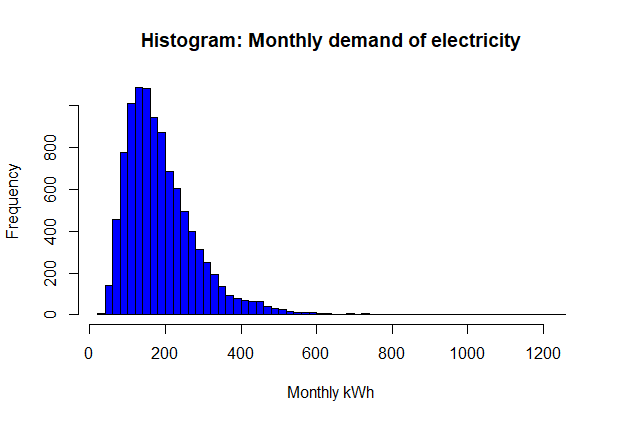
\includegraphics[width=340pt, height=200pt]{Chapters/chapter4/figures/PredDemElect.png}
	%%\centerline{\epsfig{/Chapters/chapter1/figures/cat.eps,width=.8\textheight,height=.4\textwidth}}
	\caption[List of figure caption goes here]{Histogram using the posterior predictive distribution of electricity demand}\label{fig41}
\end{figure}

 
\section{Multivariate linear regression: The conjugate normal-normal/inverse Wishart model}\label{sec44}

Let's study the multivariate regression setting where there are $N$-dimensional vectors ${\bm{y}}_m$, for $m = 1, 2, \dots, M$, such that ${\bm{y}}_m = {\bm{X}} \bm{\beta}_m + \mu_m$. Here, ${\bm{X}}$ represents the set of common regressors, and $\mu_m$ is the $N$-dimensional vector of stochastic errors for each equation. We assume that ${\bm{U}} = [\mu_1 \ \mu_2 \ \dots \ \mu_M] \sim MN_{N,M}({\bm{0}}, {\bm{I}}_N, {\bm{\Sigma}})$, which is a matrix variate normal distribution where $\bm{\Sigma}$ is the covariance matrix of each $i$-th row of ${\bm{U}}$, for $i = 1, 2, \dots, N$, and we assume independence between the rows. Consequently, we have that $vec({\bm{U}}) \sim N_{N \times M}({\bm{0}}, \bm{\Sigma} \otimes {\bm{I}}_N)$.\footnote{$vec$ denotes the vectorization operation, and $\otimes$ denotes the Kronecker product.}

This framework can be written in matrix form
\begin{align*}
	\underbrace{
		\begin{bmatrix}
			y_{11} & y_{12} & \dots & y_{1M}\\
			y_{21} & y_{22} & \dots & y_{2M}\\
			\vdots & \vdots & \dots & \vdots\\
			y_{N1} & y_{N2} & \dots & y_{NM}\\
	\end{bmatrix}}_{\bm{Y}}
	&=
	\underbrace{\begin{bmatrix}
			x_{11} & x_{12} & \dots & x_{1K}\\
			x_{21} & x_{22} & \dots & x_{2K}\\
			\vdots & \vdots & \dots & \vdots\\
			x_{N1} & x_{N2} & \dots & x_{NK}\\
	\end{bmatrix}}_{\bm{X}}
	\underbrace{
		\begin{bmatrix}
			\beta_{11} & \beta_{12} & \dots & \beta_{1M}\\
			\beta_{21} & \beta_{22} & \dots & \beta_{2M}\\
			\vdots & \vdots & \dots & \vdots\\
			\beta_{K1} & \beta_{K2} & \dots & \beta_{KM}\\
	\end{bmatrix}}_{\bm{B}}\\
	&+
	\underbrace{\begin{bmatrix}
			\mu_{11} & \mu_{12} & \dots & \mu_{1M}\\
			\mu_{21} & \mu_{22} & \dots & \mu_{2M}\\
			\vdots & \vdots & \dots & \vdots\\
			\mu_{N1} & \mu_{N2} & \dots & \mu_{NM}\\
	\end{bmatrix}}_{\bm{U}}.
\end{align*}

Therefore, ${\bm{Y}}\sim N_{N\times M}({\bm{X}}{\bm{B}},\bm{\Sigma}\otimes {\bm{I}}_N)$,\footnote{We can write down the former expression in a more familiar way using vectorization properties,
$\underbrace{vec(Y)}_{\bm{y}}=\underbrace{({\bm{I}}_M\otimes {\bm{X}})}_{{\bm{Z}}}\underbrace{vec({\bm{B}})}_{\bm{\beta}}+\underbrace{vec({\bm{U}})}_{\mu}$, where ${\bm{y}}\sim N_{N\times M}({\bm{Z}}\bm{\beta},\bm{\Sigma}\otimes {\bm{I}}_N)$.}
\begin{align*}
	p({\bm{Y}}\mid  {\bm{B}},{\bm{\Sigma}}, {\bm{X}})&\propto |{{\bm \Sigma}}|^{-N/2}\exp\left\lbrace -\frac{1}{2}tr\left[({\bm{Y}}-{\bm{X}}{\bm{B}})^{\top}({\bm{Y}}-{\bm{X}}{\bm{B}}){{\bm \Sigma}}^{-1}\right]\right\rbrace
	\\
	&=|{{\bm \Sigma}}|^{-N/2}\exp\left\lbrace -\frac{1}{2}tr\left[\left({\bm{S}}+({\bm{B}}-\widehat{\bm{B}})^{\top}{\bm{X}}^{\top}{\bm{X}}({\bm{B}}-\widehat{\bm{B}})\right){{\bm \Sigma}}^{-1}\right]\right\rbrace,
\end{align*}

where ${\bm{S}}= ({\bm{Y}}-{\bm{X}}\widehat{\bm{B}})^{\top}({\bm{Y}}-{\bm{X}}\widehat{\bm{B}})$, $\widehat{\bm{B}}= ({\bm{X}}^{\top}{\bm{X}})^{-1}{\bm{X}}^{\top}{\bm{Y}}$ (see Exercise 9).

The conjugate prior for this models is $\pi({\bm{B}},{\bm{\Sigma}})=\pi({\bm{B}}\mid {\bm{\Sigma}})\pi({\bm{\Sigma}})$ where ${\bm{B}}\mid {\bm \Sigma}\sim N_{K\times M}({\bm{B}}_{0},{\bm{V}}_{0},{\bm{\Sigma}})$ and ${\bm{\Sigma}}\sim IW({\bm{\Psi}}_{0},\alpha_{0})$, that is,
\begin{align*}
	\pi ({\bm{B}},{\bm{\Sigma}})\propto &\left|{\bm{\Sigma}} \right|^{-K/2}\exp\left\lbrace -\frac{1}{2}tr\left[({\bm{B}}-{\bm{B}}_{0})^{\top}{\bm{V}}_{0}^{-1}({\bm{B}}-{\bm{B}}_{0}){\bm \Sigma}^{-1}\right]\right\rbrace \\
	& \times \left|{\bm \Sigma} \right|^{-(\alpha_{0}+M+1)/2}\exp\left\lbrace -\frac{1}{2}tr \left[ {\bm{\Psi}}_{0} {\bm \Sigma}^{-1}\right] \right\rbrace.
\end{align*}

The posterior distribution is given by
\begin{align*}
	\pi({\bm{B}},{\bm{\Sigma}}\mid {\bm{Y}},{\bm{X}})&\propto  p({\bm{Y}}\mid {\bm{B}},{\bm{\Sigma}},{\bm{X}}) \pi({\bm{B}}\mid  {\bm \Sigma})\pi({\bm{\Sigma}})\\
	&\propto \left|{\bm{\Sigma}} \right|^{-\frac{N+K+\alpha_{0}+M+1}{2}}\\
	&\times\exp\left\lbrace -\frac{1}{2}tr\left[(\bm{\Psi}_{0}+{\bm{S}} +({\bm{B}}-{\bm{B}}_{0})^{\top}{\bm{V}}_{0}^{-1}({\bm{B}}-{\bm{B}}_{0})\right.\right.\\
	&\left.\left.   +({\bm{B}}-\widehat{\bm{B}})^{\top}{\bm{X}}^{\top}{\bm{X}}({\bm{B}}-\widehat{\bm{B}}))\bm{\Sigma}^{-1}\right]\right\rbrace .
\end{align*}
Completing the squares on ${\bm{B}}$ and collecting the remaining terms in the bracket yields
{\footnotesize{
\begin{align*}
	{\bm{\Psi}}_{0}+{\bm{S}} +({\bm{B}}-{\bm{B}}_{0})^{\top}{\bm{V}}_{0}^{-1}({\bm{B}}-{\bm{B}}_{0})+({\bm{B}}-\widehat{\bm{B}})^{\top}{\bm{X}}^{\top}{\bm{X}}({\bm{B}}-\widehat{\bm{B}})
	& = ({\bm{B}}-{\bm{B}}_n)^{\top}{\bm{V}}_n^{-1}({\bm{B}}-{\bm{B}}_n)+{\bm{\Psi}}_n,
\end{align*}
}}
where 
\begin{align*}
	{\bm{B}}_n = &({\bm{V}}_{0}^{-1}+{\bm{X}}^{\top}{\bm{X}})^{-1}({\bm{V}}_{0}^{-1}{\bm{B}}_{0}+{\bm{X}}^{\top}{\bm{Y}})=({\bm{V}}_{0}^{-1}+{\bm{X}}^{\top}{\bm{X}})^{-1}({\bm{V}}_{0}^{-1}{\bm{B}}_{0}+{\bm{X}}^{\top}{\bm{X}}\widehat{\bm{B}}),\\
	{\bm{V}}_n = &({\bm{V}}_{0}^{-1}+{\bm{X}}^{\top}{\bm{X}})^{-1},\\
	{\bm{\Psi}}_n= &{\bm{\Psi}}_{0}+{\bm{S}}+{\bm{B}}_{0}^{\top}{\bm{V}}_{0}^{-1}{\bm{B}}_{0}+\widehat{\bm{B}}^{\top}{\bm{X}}^{\top}{\bm{X}}\widehat{\bm{B}}-{\bm{B}}_n^{\top}{\bm{V}}_n^{-1}{\bm{B}}_n.
\end{align*}
Thus, the posterior distribution can be written as
\begin{align*}
	\pi({\bm{B}},{\bm \Sigma}\mid  {\bm{Y}}, {\bm{X}})\propto &\left|{\bm \Sigma} \right|^{-K/2}\exp\left\lbrace -\frac{1}{2} tr\left[({\bm{B}}-{\bm{B}}_n)^{\top}{\bm{V}}_n^{-1}({\bm{B}}-{\bm{B}}_n)   {\bm \Sigma}^{-1}\right]\right\rbrace \\
	\times & \left|{\bm \Sigma} \right|^{-\frac{N+\alpha_{0}+M+1}{2}}\exp\left\lbrace -\frac{1}{2} tr \left[ {\bm{\Psi}}_n{\bm \Sigma}^{-1}\right] \right\rbrace .
\end{align*}
That is $\pi({\bm{B}},{\bm \Sigma}\mid  {\bm{Y}}, {\bm{X}})=\pi ({\bm{B}}\mid  {\bm \Sigma},{\bm{Y}},{\bm{X}})\pi({\bm \Sigma}\mid  {\bm{Y}},{\bm{X}})$ where ${\bm{B}}\mid  {\bm \Sigma},{\bm{Y}}, {\bm{X}} \sim N_{K\times M}({\bm{B}}_n,{\bm{V}}_n,{\bm \Sigma})$ and ${\bm \Sigma}\mid  {\bm{Y}},{\bm{X}} \sim IW({\bm{\Psi}}_n,{\alpha}_n)$, $\alpha_n= N+\alpha_{0}$. Observe again that we can write down the posterior mean as a weighted average between prior and sample information such that ${\bm{V}}_0\rightarrow\infty$ implies ${\bm{B}}_n\rightarrow\hat{{\bm{B}}}$, as we show in the univariate linear model.

The marginal posterior for ${\bm{B}}$ is given by
\begin{align*}
	\pi({\bm{B}}\mid {\bm{Y}},{\bm{X}})&\propto \int_{\bm{\mathcal{S}}} \left|{\bm \Sigma} \right|^{-(\alpha_n+K+M+1)/2}\\
	&\times\exp\left\lbrace -\frac{1}{2} tr\left\{\left[({\bm{B}}-{\bm{B}}_n)^{\top}{\bm{V}}_n^{-1}({\bm{B}}-{\bm{B}}_n)+{\bm{\Psi}}_n \right]  {\bm \Sigma}^{-1}\right\}\right\rbrace d{\bm{\Sigma}} \\
 	&\propto|({\bm{B}}-{\bm{B}}_n)^{\top}{\bm{V}}_n^{-1}({\bm{B}}-{\bm{B}}_n)+{\bm{\Psi}}_n|^{-(K+\alpha_n)/2}\\
 	&=\left[|{\bm{\Psi}}_n|\times|{\bm{I}}_K+{\bm{V}}_n^{-1}({\bm{B}}-{\bm{B}}_n){\bm{\Psi}}_n^{-1}({\bm{B}}-{\bm{B}}_n)^{\top}|\right]^{-(\alpha_n+1-M+K+M-1)/2}\\
 	&\propto|{\bm{I}}_K+{\bm{V}}_n^{-1}({\bm{B}}-{\bm{B}}_n){\bm{\Psi}}_n^{-1}({\bm{B}}-{\bm{B}}_n)^{\top}|^{-(\alpha_n+1-M+K+M-1)/2}.
\end{align*}

The second line uses the inverse Wishart distribution, the third line the Sylverter's theorem, and the last line is the kernel of a matrix $t$-distribution, that is, ${\bm{B}}\mid {\bm{Y}},{\bm{X}}\sim T_{K\times M}({\bm{B}}_n,{\bm{V}}_n,{\bm{\Psi}}_n)$ with $\alpha_n+1-M$ degrees of freedom. 

Observe that $vec({\bm{B}})$ has mean $vec({\bm{B}}_n)$ and variance $({\bm{V}}_n\otimes{\bm{\Psi}}_n)/(\alpha_n-M-1)$ based on its marginal distribution. On the other hand, the variance based on the conditional distribution is ${\bm{V}}_n\otimes{\bm{\Sigma}}$, where the mean of ${\bm{\Sigma}}$ is ${\bm{\Psi}}_n/(\alpha_n-M-1)$.   

The marginal likelihood is the following,
\begin{align*}
	p({\bm{Y}})&=\int_{\mathcal{B}}\int_{\mathcal{S}}\left\{ (2\pi)^{-NM/2} |{{\bm \Sigma}}|^{-N/2}\exp\left\lbrace -\frac{1}{2}tr\left[{\bm{S}}+({\bm{B}}-\widehat{\bm{B}})^{\top}{\bm{X}}^{\top}{\bm{X}}({\bm{B}}-\widehat{\bm{B}})\right]{{\bm \Sigma}}^{-1}\right\rbrace\right.\\
	&\times (2\pi)^{-KM/2}\left|{\bm V}_0 \right|^{-M/2} \left|{\bm{\Sigma}} \right|^{-K/2}\exp\left\lbrace -\frac{1}{2}tr\left[({\bm{B}}-{\bm{B}}_{0})^{\top}{\bm{V}}_{0}^{-1}({\bm{B}}-{\bm{B}}_{0}){\bm \Sigma}^{-1}\right]\right\rbrace \\
	&\left. \times \frac{|\Psi_0|^{\alpha_0/2}}{2^{\alpha_0M/2}\Gamma_M(\alpha_0/2)} \left|{\bm \Sigma} \right|^{-(\alpha_{0}+M+1)/2}\exp\left\lbrace -\frac{1}{2}tr \left[ {\bm{\Psi}}_{0} {\bm \Sigma}^{-1}\right] \right\rbrace \right\} d{\bm{\Sigma}} d{\bm B}\\
	&=(2\pi)^{-M(N+K)/2}\left|{\bm V}_0\right|^{-M/2}\frac{|\Psi_0|^{\alpha_0/2}}{2^{\alpha_0M/2}\Gamma_M(\alpha_0/2)}\\
	&\times\int_{\mathcal{B}}\int_{\mathcal{S}} \left\{ \left|{\bm \Sigma} \right|^{-(\alpha_{0}+N+K+M+1)/2}\right.\\
	&\left. \exp\left\lbrace -\frac{1}{2}tr\left[{\bm{S}}+({\bm{B}}-\widehat{\bm{B}})^{\top}{\bm{X}}^{\top}{\bm{X}}({\bm{B}}-\widehat{\bm{B}})+({\bm{B}}-{\bm{B}}_{0})^{\top}{\bm{V}}_{0}^{-1}({\bm{B}}-{\bm{B}}_{0})+{\bm{\Psi}}_0\right]{{\bm \Sigma}}^{-1}\right\rbrace\right\}d{\bm{\Sigma}} d{\bm B}\\
	&=(2\pi)^{-M(N+K)/2}\left|{\bm V}_0\right|^{-M/2}\frac{|\Psi_0|^{\alpha_0/2}}{2^{\alpha_0M/2}\Gamma_M(\alpha_0/2)}2^{M(\alpha_n+K)/2}\Gamma_M((\alpha_n+K)/2)\\
	&\times \int_{\mathcal{B}}\left|{\bm{S}}+({\bm{B}}-\widehat{\bm{B}})^{\top}{\bm{X}}^{\top}{\bm{X}}({\bm{B}}-\widehat{\bm{B}})+({\bm{B}}-{\bm{B}}_{0})^{\top}{\bm{V}}_{0}^{-1}({\bm{B}}-{\bm{B}}_{0})+{\bm{\Psi}}_0\right|^{-(\alpha_n+K)/2}d{\bm{B}}\\
	&=(2\pi)^{-M(N+K)/2}\left|{\bm V}_0\right|^{-M/2}\frac{|\Psi_0|^{\alpha_0/2}}{2^{\alpha_0M/2}\Gamma_M(\alpha_0/2)}2^{M(\alpha_n+K)/2}\Gamma_M((\alpha_n+K)/2)\\
	&\times \int_{\mathcal{B}}\left|({\bm{B}}-\widehat{\bm{B}}_n)^{\top}{\bm{V}}_n^{-1}({\bm{B}}-\widehat{\bm{B}}_n)+{\bm{\Psi}}_n\right|^{-(\alpha_n+K)/2}d{\bm{B}}\\ 
	&=(2\pi)^{-M(N+K)/2}\left|{\bm V}_0\right|^{-M/2}\frac{|\Psi_0|^{\alpha_0/2}}{2^{\alpha_0M/2}\Gamma_M(\alpha_0/2)}2^{M(\alpha_n+K)/2}\Gamma_M((\alpha_n+K)/2)\\
	&\times \int_{\mathcal{B}}\left[|{\bm{\Psi}}_n|\times |{\bm{I}}_{K}+{\bm{V}}_n^{-1}({\bm{B}}-\widehat{\bm{B}}_n){\bm{\Psi}}_n^{-1}({\bm{B}}-\widehat{\bm{B}}_n)^{\top}|\right]^{-(\alpha_n+K)/2}d{\bm{B}}\\
	&=|{\bm{\Psi}}_n|^{-(\alpha_n+K)/2}(2\pi)^{-M(N+K)/2}\left|{\bm V}_0\right|^{-M/2}\frac{|\Psi_0|^{\alpha_0/2}2^{M(\alpha_n+K)/2}\Gamma_M((\alpha_n+K)/2)}{2^{\alpha_0M/2}\Gamma_M(\alpha_0/2)}\\
	&\times \int_{\mathcal{{\bm{B}}}}\left| {\bm{I}}_{K}+{\bm{V}}_n^{-1}({\bm{B}}-\widehat{\bm{B}}_n){\bm{\Psi}}_n^{-1}({\bm{B}}-\widehat{\bm{B}}_n)^{\top}\right|^{-(\alpha_n+1-M+K+M-1)/2}d{\bm{B}}\\
	&=|{\bm{\Psi}}_n|^{-(\alpha_n+K)/2}(2\pi)^{-M(N+K)/2}\left|{\bm V}_0\right|^{-M/2}\frac{|\Psi_0|^{\alpha_0/2}2^{M(\alpha_n+K)/2}\Gamma_M((\alpha_n+K)/2)}{2^{\alpha_0M/2}\Gamma_M(\alpha_0/2)}\\
	&\times \pi^{MK/2}\frac{\Gamma_M((\alpha_n+1-M+M-1)/2)}{\Gamma_M((\alpha_n+1-M+K+M-1)/2)}|{\bm{\Psi}}_n|^{K/2}|{\bm{V}}_n|^{M/2}\\
	&=\frac{|{\bm{V}}_n|^{M/2}}{|{\bm{V}}_0|^{M/2}}\frac{|{\bm{\Psi}}_0|^{\alpha_0/2}}{|{\bm{\Psi}}_n|^{\alpha_n/2}}\frac{\Gamma_M(\alpha_n/2)}{\Gamma_M(\alpha_0/2)}\pi^{-MN/2}.  
\end{align*}

The third equality follows from the kernel of an inverse Wishart distribution, the fifth from Sylvester's theorem, and the seventh from the kernel of a matrix $t$-distribution.

Observe that this last expression is the multivariate case of the marginal likelihood of the univariate regression model. Taking into account that 
\begin{align*}
	({\bm{A}}+{\bm{B}})^{-1}&={\bm{A}}^{-1}-({\bm{A}}^{-1}+{\bm{B}}^{-1})^{-1}{\bm{A}}^{-1}\\
	&={\bm{B}}^{-1}-({\bm{A}}^{-1}+{\bm{B}}^{-1})^{-1}{\bm{B}}^{-1}\\
	&={\bm{A}}^{-1}({\bm{A}}^{-1}+{\bm{B}}^{-1}){\bm{B}}^{-1},
\end{align*} 

we can show that ${\bm{\Psi}}_{n}={\bm{\Psi}}_{0}+{\bm{S}}+(\hat{\bm{B}}-{\bm{B}}_{0})^{\top}{\bm{V}}_{n}(\hat{\bm{B}}-{\bm{B}}_{0})$ (see Exercise 7). Therefore, the marginal likelihood rewards fit (smaller sum of squares, ${\bm{S}}$), similarity between prior and sample information regarding location parameters, and information gains in variability from ${\bm{V}}_0$ to ${\bm{V}}_n$.   

Given a matrix of regressors ${\bm{X}}_0$ for $N_0$ unobserved units, the predictive density of ${\bm{Y}}_0$ given ${\bm{Y}}$, $\pi({\bm{Y}}_0\mid {\bm{Y}})$ is a matrix t distribution $T_{N_0,M}(\alpha_n-M+1,{\bm{X}}_0{\bm{B}}_n,{\bm{I}}_{N_0}+{\bm{X}}_0{\bm{V}}_n{\bm{X}}_0^{\top},{\bm{\Psi}}_n)$ (see Exercise 6). Observe that the prediction is centered at ${\bm{X}}_0{\bm{B}}_n$, and the covariance matrix of $vec({\bm{Y}}_0)$ is $\frac{({\bm{I}}_{N_0}+{\bm{X}}_0{\bm{V}}_n{\bm{X}}_0^{\top})\otimes{\bm{\Psi}}_n}{\alpha_n-M-1}$.  

\section{Summary}\label{sec45}
We introduce conjugate family models for both discrete and continuous data. These models form the foundation of the Bayesian framework due to their mathematical tractability, as they provide closed-form expressions for the posterior distributions, marginal likelihood, and predictive distribution. Additionally, we present the Bayesian linear regression frameworks for both univariate and multivariate cases under conjugate families. These frameworks are fundamental for performing regression analysis in the Bayesian setting.

\section{Exercises}\label{sec46}

\begin{enumerate}
	\item Write the distribution of the Bernoulli example in canonical form, and find the mean and variance of the sufficient statistic.
	
	\item Given a random sample \(\bm{Y} = [Y_1 \ Y_2 \ \dots \ Y_N]^{\top}\) from \(N\) \textit{binomial experiments}, each with known size \(n_i\) and the same unknown probability \(\theta\), show that \(p(\bm{y} \mid \theta)\) is in the exponential family. Then, find the posterior distribution, the marginal likelihood, and the predictive distribution of the binomial-Beta model assuming the number of trials is known.
	
	\item Given a random sample \(\bm{Y} = [Y_1 \ Y_2 \ \dots \ Y_N]^{\top}\) from an \textit{exponential distribution}, show that \(p(\bm{y} \mid \lambda)\) is in the exponential family. Additionally, find the posterior distribution, the marginal likelihood, and the predictive distribution of the exponential-Gamma model.
	
	\item Given that \(\bm{Y} \sim N_N(\bm{\mu}, \bm{\Sigma})\), that is, a \textit{multivariate normal distribution}, show that \(p(\bm{y} \mid \bm{\mu}, \bm{\Sigma})\) is in the exponential family.
	
	\item Find the marginal likelihood in the normal/inverse-Wishart model.
		
	\item Find the posterior predictive distribution in the normal/inverse-Wishart model, and show that ${\bm{Y}}_0\mid {\bm{Y}}\sim T_{N_0,M}(\alpha_n-M+1,{\bm{X}}_0{\bm{B}}_n,{\bm{I}}_{N_0}+{\bm{X}}_0{\bm{V}}_n{\bm{X}}_0^{\top},{\bm{\Psi}}_n)$.
	
	\item Show that $\delta_n=\delta_0+({\bm{y}}-{\bm{X}}\hat{\bm{\beta}})^{\top}({\bm{y}}-{\bm{X}}\hat{\bm{\beta}})+(\hat{\bm{\beta}}-\bm{\beta}_0)^{\top}(({\bm{X}}^{\top}{\bm{X}})^{-1}+{\bm{B}}_0)^{-1}(\hat{\bm{\beta}}-\bm{\beta}_0)$ in the linear regression model, and that ${\bm{\Psi}}_{n}={\bm{\Psi}}_{0}+{\bm{S}}+(\hat{\bm{B}}-{\bm{B}}_{0})^{\top}{\bm{V}}_{n}(\hat{\bm{B}}-{\bm{B}}_{0})$ in the linear multivariate regression model. 
			
	\item Show that in the linear regression model $\bm{\beta}_n^{\top}({\bm{B}}_n^{-1}-{\bm{B}}_n^{-1}{\bm{M}}^{-1}{\bm{B}}_n^{-1})\bm{\beta}_n={\bm{\bm{\beta}}}_{**}^{\top}{\bm{C}}{\bm{\bm{\beta}}}_{**}$ and $\bm{\beta}_{**}={\bm{X}}_0\bm{\beta}_n$.
	
	\item Show that $({\bm{Y}}-{\bm{X}}{\bm{B}})^{\top}({\bm{Y}}-{\bm{X}}{\bm{B}})={\bm{S}}+({\bm{B}}-\widehat{\bm{B}})^{\top}{\bm{X}}^{\top}{\bm{X}}({\bm{B}}-\widehat{\bm{B}})$ where ${\bm{S}}= ({\bm{Y}}-{\bm{X}}\widehat{\bm{B}})^{\top}({\bm{Y}}-{\bm{X}}\widehat{\bm{B}})$, $\widehat{\bm{B}}= ({\bm{X}}^{\top}{\bm{X}})^{-1}{\bm{X}}^{\top}{\bm{Y}}$ in the multivariate regression model.
	
	\item \textbf{What is the probability that the Sun will rise tomorrow?}
	
	This is the most famous example by Richard Price, developed in the Appendix of Bayes' theorem paper \cite{bayes1763lii}. Here, we implicitly use \textit{Laplace's Rule of Succession} to solve this problem. In particular, if we were a priori uncertain about the probability that the Sun will rise on a specified day, we can assume a uniform prior distribution over \((0,1)\), that is, a Beta(1,1) distribution. Then, what is the probability that the Sun will rise?
	
	\item Using information from Public Policy Polling in September 27th-28th for the 2016 presidential five-way race in USA, there are 411, 373 and 149 sampled people supporting Hillary Clinton, Donald Trump and other, respectively. 
	
	\begin{itemize}
		\item Find the posterior probability of the percentage difference of people supporting Hillary versus Trump according to this data using a non-informative prior, that is, $\alpha_0=[1 \ 1 \ 1]$ in the multinomial-Dirichlet model. What is the probability of having more supports of Hillary vs Trump?
		
		\item What is the probability that sampling one hundred independent individuals 44, 40 and 16 support Hillary, Trump and other, respectively?  
	\end{itemize}

\item \textbf{Math test example continues}

You have a random sample of math scores of size $N=50$ from a normal distribution, $Y_i\sim {N}(\mu, \sigma^2)$. The sample mean and variance are equal to $102$ and $10$, respectively. Using the normal-normal/inverse-gamma model where $\mu_0=100$, $\beta_0=1$, $\alpha_0=\delta_0=0.001$

\begin{itemize}
	\item Get a 95\% confidence and credible interval for $\mu$.
	\item What is the posterior probability that $\mu > 103$?  
\end{itemize} 

%\item In the optimal tangency portfolio example, what are the equations for $\mu_{T+\kappa}=\mu_n$ and ${\bm{\Sigma}}_{T+\kappa}$? Use these equations to find the optimal weights six periods ahead using the tech stocks. 

\item \textbf{Demand of electricity example continues}

Set $c_0$ such that maximizes the marginal likelihood in the specifications with and without electricity price in the example of demand of electricity (empirical Bayes). Then, calculate the Bayes factor, and conclude if there is evidence supporting the inclusion of the price of electricity in the demand equation.

\item \textbf{Utility demand}

Use the file \textit{Utilities.csv} to estimate a multivariate linear regression model where $\bm{Y}_i=\left[\log(\text{electricity}_i) \ \log(\text{water}_i) \ \log(\text{gas}_i)\right]$ as function of $\log(\text{electricity price}_i)$, $\log(\text{water price}_i)$, $\log(\text{gas price}_i)$, $\text{IndSocio1}_i$, $\text{IndSocio2}_i$, $\text{Altitude}_i$, $\text{Nrooms}_i$, $\text{HouseholdMem}_i$, $\text{Children}_i$, and $\log(\text{Income}_i)$, where electricity, water and gas are monthly consumption of electricity (kWh), water (m$^3$) and gas (m$^3$), and other definitions are given in the Example of Section \ref{sec43}. Omit households that do not consume any of the utilities in this exercise.  

Set a non-informative prior framework, $\bm{B}_0=\left[0\right]_{11\times 3}$, $\bm{V}_0=1000 \bm{I}_{11}$, $\bm{\Psi}_0=1000 \bm{I}_{3}$ and $\alpha_0=3$, where we have $K=11$ (regressors plus intercept) and $M=3$ (equations) in this exercise.

\begin{itemize}
	\item Find the posterior mean estimates and the highest posterior density intervals at 95\% of $\bm{B}$ and $\bm{\Sigma}$. Use the marginal distribution and the conditional distribution to obtain the posterior estimates of  $\bm{B}$, and compare the results.
	\item Find the Bayes factor comparing the baseline model in this exercise with the same specification but using the income in dollars. Now, calculate the Bayes factor using the income in thousand dollars. Is there any difference?
	\item Find the predictive distribution for the monthly demand of electricity, water and gas in the baseline specification of a household located in the lowest socioeconomic condition in a municipality located below 1000 meters above the sea level, 2 rooms, 3 members with children, a monthly income equal to USD 500, an electricity price equal to USD/kWh 0.15, a water price equal to USD/M$^3$ 0.70, and a gas price equal to USD/M$^3$ 0.75. 
\end{itemize} 

\item \textbf{Ph.D. students sleeping hours \cite[Chap.~2]{albert2009bayesian}}

We are interested in learning about the proportion of Ph.D. students who sleep at least 6 hours per day. We have a sample of 52 students, where 15 report sleeping at least 6 hours, and the remaining 37 report not sleeping at least 6 hours. The prior distribution is a Beta distribution, with hyperparameters calibrated so that the prior probabilities of the proportion of students who sleep least than 6 hours being less than 0.4 and 0.75 are 0.6 and 0.95, respectively. Estimate the 95\% posterior credible interval for the proportion of Ph.D. students who sleep at least 6 hours per day. Then, assume there is a group of experts whose beliefs about the proportion of Ph.D. students sleeping at least 6 hours are represented in the following table:

\begin{table}[!htbp]%1
	%\noautomaticrules
	\tabletitle{Probability distribution: Ph.D students that sleep at least 6 hours per day.}\label{tab:sleep}%
	\begin{tabular}{cccccccccccc}
		$h$   & 0.05 & 0.10 & 0.15 & 0.20 & 0.25 & 0.30 & 0.35 & 0.40 & 0.45 & 0.50 & 0.55  \\
		\hline
		$P(p=h)$ & 0.05 & 0.07 & 0.10 & 0.12 & 0.15 & 0.17 & 0.15 & 0.11 & 0.06 & 0.01 & 0.01 \\ 

	\end{tabular}
%	\begin{tablenotes}[para,flushleft]
%		\footnotesize \textit{Notes}: Hypothetical distribution of Ph.D. students that sleep at least 6 hours per day.\\
%	\end{tablenotes}
\end{table}
Use Table \ref{tab:sleep} as prior information, and find the posterior distribution of the proportion of students that sleep at least 6 hours. 
	

\end{enumerate}



